\section{Geometric Centres}

\subsection{Median and Centroid}

Median (notice the "mid") is the line from one vertex of a triangle to one edge of the triangle such that it divides the edge in two equal parts \\

\begin{figure*}[h!]
    \centering
    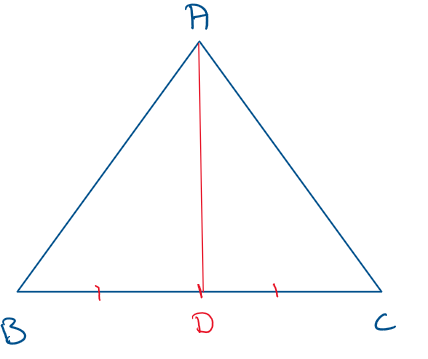
\includegraphics[width=0.25\linewidth]{Quant//Geometry//Images//Triangles/triangle_median_intro.png}
\end{figure*}


$AD$ is the median of side $BC$ and $BD = CD$. Note that \textbf{median is not necessarily a perpendicular to the side} 

A centroid is the intersection of all medians of a triangle. 

\begin{figure*}[h!]
    \centering
    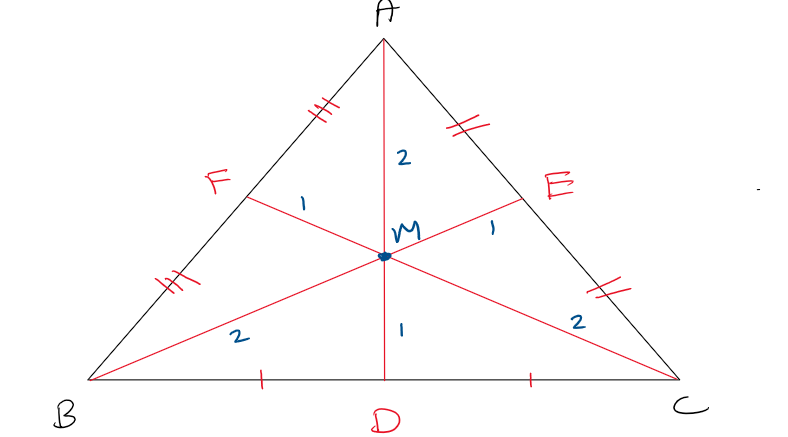
\includegraphics[width=0.4\linewidth]{Quant//Geometry//Images//Triangles/triangle_centroid_intro.png}    
\end{figure*}
        

A centroid divides the medians in the ratio of 2:1 from the vertex of median
\begin{itemize}
    \item $AM : MD = 2 : 1$
    \item $BM : ME = 2 : 1$
    \item $CM : MF = 2 : 1$
\end{itemize}
It divides the triangle into 6 triangles of equal area $\implies$ AMF = AME = BMF = BMD = CMD = CEF in terms of area

\subsection{Altitude and Orthocenter}
An altitude (perpendicular) is a vertical line from vertex to edge of a triangle. It makes an angle of 90 degree (right angle) with the base. \textbf{Perpendicular is not median}. As we can see, $AD$ is altitude (as it makes an angle of $\degree{90}$ with the base and $AM$ is the median. 

\begin{figure*}[h!]
    \centering
    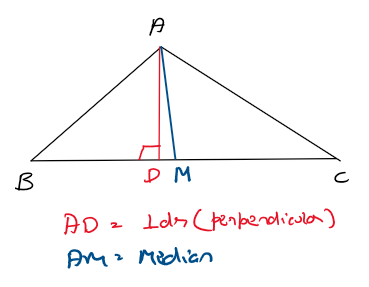
\includegraphics[width=0.5\linewidth]{Quant//Geometry//Images//Triangles/altitude.png}
\end{figure*}

Orthocenter of a triangle is the point of intersection of altitudes made from each vertex of triangle to its corresponding edge. In the figure below, $O$ is the orthocenter. 

\begin{figure*}[h!]
    \centering
    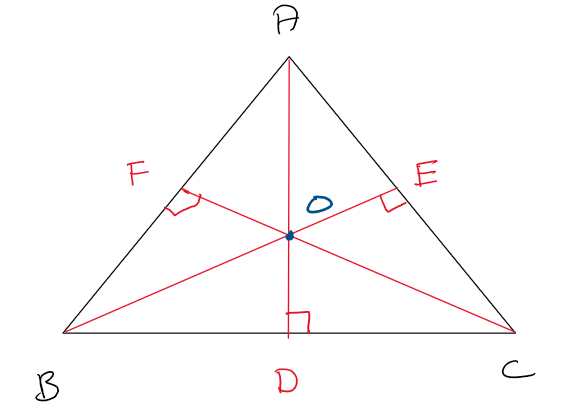
\includegraphics[width=0.5\linewidth]{Quant//Geometry//Images//Triangles/orthocenter.png}
\end{figure*}

A \textbf{property of orthocenter} : The sum of angles between two vertex and orthocentre and the angle of other vertex is always 180 degree. From this, we can say that in the above figure
\begin{itemize}
    \item $\angle A + \angle BOC = \degree{180}$
    \item $\angle B + \angle AOC = \degree{180}$
    \item $\angle C + \angle AOB = \degree{180}$
\end{itemize}

\subsection{Angle Bisector and Incenter}
Angle bisector is drawn from vertex of triangle to the adjacent side. This line divides the angle at the vertex in two equal angles

\begin{figure*}[h!]
    \centering
    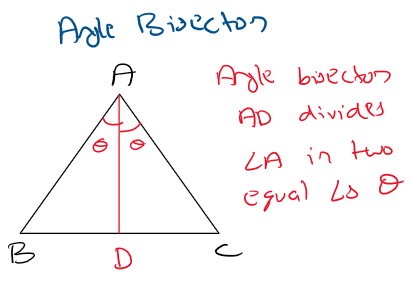
\includegraphics[width=0.5\linewidth]{Quant//Geometry//Images//Triangles/angle_bisector.png}
\end{figure*}

Incentre (Incenter) is the point at which the angle bisectors of each vertex of triangle intersect. This point is denoted as $I$. In the below figure, $AD, BE, CF$ are angle bisectors

\begin{figure*}[h!]
    \centering
    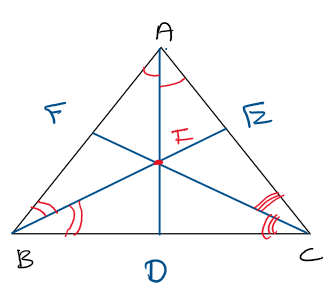
\includegraphics[width=0.5\linewidth]{Quant//Geometry//Images//Triangles/incenter.png}
\end{figure*}

\textbf{Property} : The angle made between an edge and incenter is related to the angle of the other vertex are as follows:
\begin{itemize}
    \item $\angle BIC = 90 + \dfrac{\angle A}{2}$
    \item $\angle AIC = 90 + \dfrac{\angle B}{2}$
    \item $\angle AIB = 90 + \dfrac{\angle C}{2}$
\end{itemize}

\subsection{Perpendicular Side Bisectors and Circumcenter}
Perpendicular Side Bisector is the line which divides a line in two equal parts at a right angle. In the triangle below, $DX$ is the perpendicular bisector of $BC$ which divides $BC$ into $BX \text{ and } CX \text{ where } BX = CX$

\begin{figure*}[h!]
    \centering
    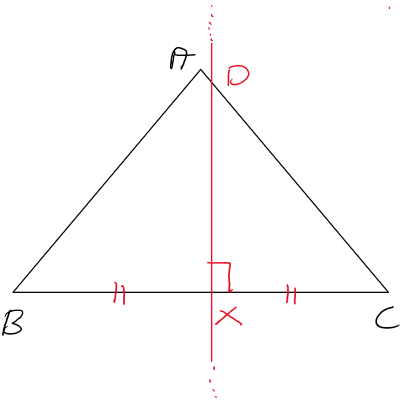
\includegraphics[width=0.5\linewidth]{Quant//Geometry//Images//Triangles/perpendicular_side_bisector.png}
\end{figure*}

Circumcenter is the point where perpendicular side bisectors of the three sides of a triangle intersect. In the triangle below, it is denoted as $O$

\begin{figure*}[h!]
    \centering
    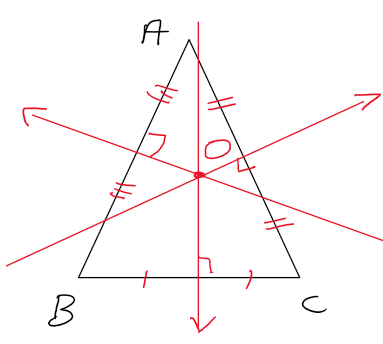
\includegraphics[width=0.5\linewidth]{Quant//Geometry//Images//Triangles/circumcenter.png}
\end{figure*}

\newpage

\subsection{Incircle and Circumcircle}

\subsubsection{Incircle}
We can make a circle inside a triangle by keeping the incenter as origin. This circle will intersect the triangle at three points. The radius of incircle is denoted by $r$. Note that in the below figure, $IX = IY = IZ = r$

\begin{figure*}[h!]
    \centering
    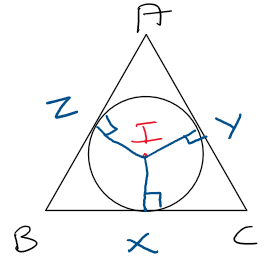
\includegraphics[width=0.4\linewidth]{Quant//Geometry//Images//Triangles/incircle.png}    
\end{figure*}

A circle's radius is perpendicular to its tangents. In this case
\begin{itemize}
    \item $IY$ is perpendicular to $AC$ ($AC$ is tangent)
    \item $IX$ is perpendicular to $BC$ ($BC$ is tangent)
    \item $IZ$ is perpendicular to $BA$ ($BA$ is tangent)
\end{itemize}

\subsubsection{Circumcircle}
We can draw a circle using this circumcenter. This circle will cover the full triangle. There is an interesting property : The circumcenter $O$ is equidistant from vertices of Triangle $\implies OA = OB = OC = R$

\begin{figure*}[h!]
    \centering
    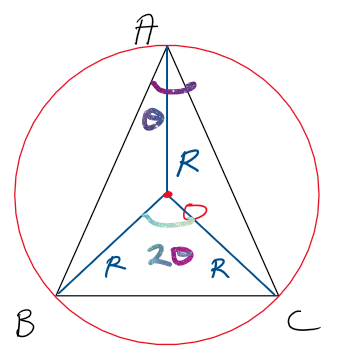
\includegraphics[width=0.38\linewidth]{Quant//Geometry//Images//Triangles/circumcircle.png}
\end{figure*}

This is a property of circles and sectors that is applicable to circumcircle..
$$
\angle BOC = 2 * \angle A
$$

\subsubsection{Distance between circumcenter and incenter}
The distance $d$ between Cirucmcenter with radius (called \textbf{circumradius}) $R$ and incenter with radius (called \textbf{inradius}) $r$ is defined as $d^2 = R * (R - 2r)$ \\

We can use the above formula to derive a relation between Inradius and circumradius as follows
\begin{align*}
    d^2 &\geq 0 \tag{Square of a number is always positive} \\
    R * (R - 2r) &\geq 0 \\
    R - 2r &\geq 0 \\
    \dfrac{R}{r} &\geq 2 \tag{$\dfrac{R}{r} = 2$ if triangle is equilateral}
\end{align*}

\SampleQuestion{In $\Triangle{ABC}$, $O$ is the point of intersection of altitudes and $I$ is the point of intersection of angle bisectors. If $\angle BOC = \degree{112}$, then find $\angle BIC$}

\begin{figure*}[h!]
    \centering
    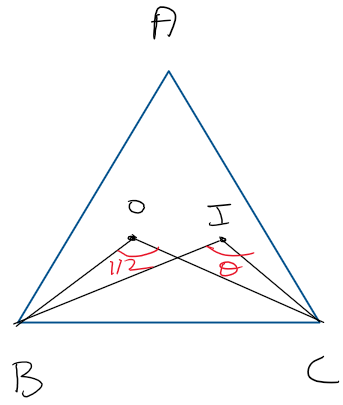
\includegraphics[width=0.3\linewidth]{Quant//Geometry//Images//Triangles/geo_center_question_1.png}
\end{figure*}

\begin{align*}
    \angle A + \angle BOC &= \degree{180} \tag{Property of orthocenter} \\
    \angle A &= \degree{68} \\
    \shortintertext{Now, using the above, we can find the value of $\angle BIC$} \\
    \angle BIC &= 90 + \dfrac{\angle A}{2} + 90 \tag{Property of incenter} \\
    &= \degree{124}
\end{align*}








\newpage

\section{Appollonius Theorem and Results}

\subsection*{Theorem}

This theorem is used to relate medians and triangles. The base theorem is that the median , the side on which we have drawn the median and the other sides of triangles are related

\begin{figure*}[h!]
    \centering
    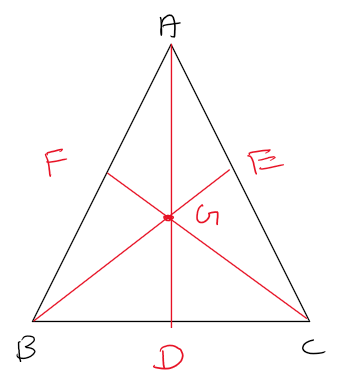
\includegraphics[width=0.3\linewidth]{Quant//Geometry//Images//Triangles/appollonius_figure.png}
\end{figure*}

For the above figure and medians, we have the following equations

\begin{table}[h!]
    \centering
    \begin{tabular}{|| c | c | c | c | p{3cm} ||}
        \hline
         Median & Base & Other Sides & Relation & Alternative \\
         \hline
         $AD$ & $BC$ & $AB,AC$ & $2 * (AD^2 + CD^2 ) = AB^2 + AC^2$ & Instead of $CD$, we can also use $BD$) \\
         \hline
         $BE$ & $AC$ & $AB,BC$ & $2 * (BE^2 + CE^2 ) = AB^2 + BC^2$ & Instead of $CE$, we can also use $AE$) \\
         \hline
         $CF$ & $AB$ & $AC,BC$ & $2 * (CF^2 + AF^2 ) = AC^2 + BC^2$ & Instead of $AF$, we can also use $BF$) \\
         \hline
    \end{tabular}
\end{table}

\subsection*{Results}

\begin{itemize}
    \item $\dfrac{\text{Sum of square of medians of triangle}}{\text{Sum of square of sides of triangle}} = \dfrac{3}{4}$

    \item Sum of medians $<$ Perimeter of Triangle $< \dfrac{4}{3}$ Sum of medians
    \item The centroid divides a median in the ratio $2 : 1$. For the sake of below formula, let us refer the sides as "bigger side" and "smaller side"... 
    $$
    \dfrac{ \text{Sum of square of bigger sides of median} }{ \text{Sum of square of sides of triangle} } = \dfrac{1}{3}
    $$
\end{itemize}

\newpage 

\section{Area of Triangle}
\subsection{Heron's Formula}

In the triangle with lengths of sides as $a,b,c$, we can find area using the formula below

\begin{figure*}[h!]
    \centering
    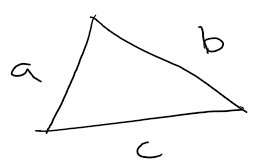
\includegraphics[width=0.4\linewidth]{Quant//Geometry//Images//Triangles/herons.png}
\end{figure*}

Area = $\sqrt{ s * (s - a) * (s - b) * (s - c) }$, $s = \dfrac{a + b + c}{2}$

\subsection{Using base and height}

The formula is $\dfrac{1}{2} * \text{base} * \text{height}$. The important thing is to determine correctly which dimension is the base and which is the height. 

\begin{figure*}[h!]
    \centering
    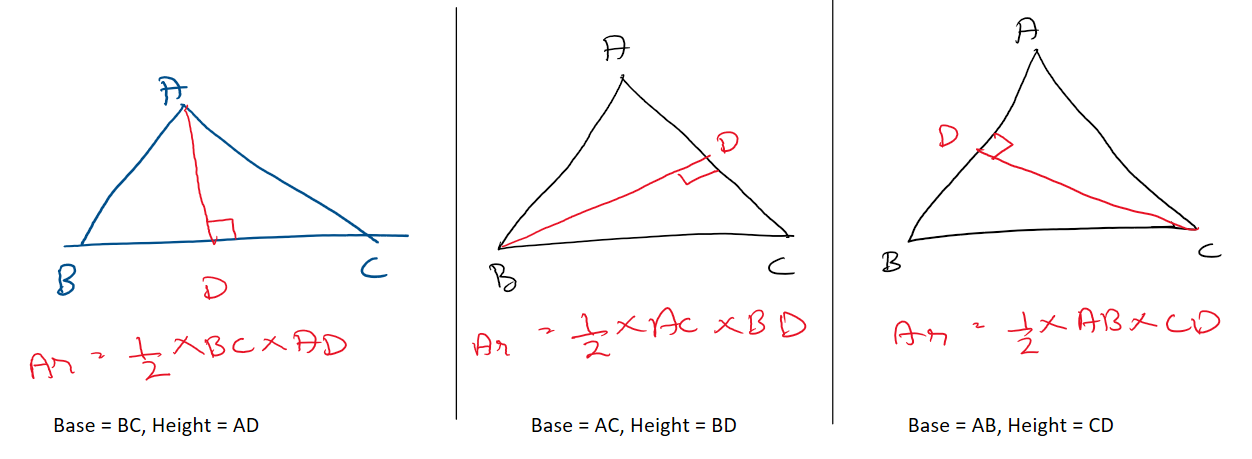
\includegraphics[width=1.0\linewidth]{Quant//Geometry//Images//Triangles/half_base_height.png}
\end{figure*}


\subsection{Using Inradius and Circumradius}

For a triangle with dimensions as $a,b,c$, its area with respect to incenter and circumcenter is summarised in below table

\begin{table}[h!]
    \centering
    \begin{tabular}{|| c | c | c | c ||}
        \hline
         Radius & Represented as & Formula & Note \\
        \hline
         Inradius & $r$ & $r * s$ & $s = \dfrac{a + b + c}{2}$ \\
        \hline
         Circumradius & $R$ & $\dfrac{abc}{4R}$ & \\
        \hline
    \end{tabular}
\end{table}

\subsection{Using Trigonometery}
We can also using trigonometery to calculate area of triangle. We will consider any two sides of triangle and the angle between them. 

\begin{figure*}[h!]
    \centering
    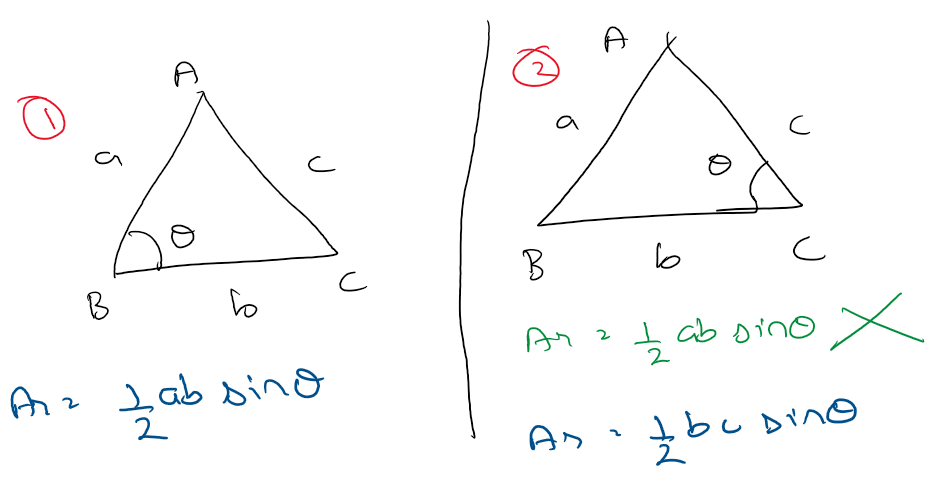
\includegraphics[width=0.9\linewidth]{Quant//Geometry//Images//Triangles/area_trigo.png}
\end{figure*}

\begin{itemize}
    \item In case 1, the angle $\theta$ between sides $a$ and $b$ is considered. The area is $\dfrac{1}{2} * a * b * \sin{\theta} $

    \item In case 2, the angle $\theta$ between sides $b$ and $C$ \textbf{should be considered.} . The area is $\dfrac{1}{2} * b * c * \sin{\theta} $
    
\end{itemize}


\subsection{Area of triangle made by median}
For a triangle ABC, when the length of the medians $AD, BE, CF$ are given, then if we arrange the medians in such a way that they make a triangle DEF, then area of ABC and DEF are related as follows

$$
\Area{DEF} = \dfrac{3}{4} \Area{ABC}
$$

\SampleQuestion{$AD = 9, BE = 12, CF = 15$. $AD,BE \& CF$ are medians of $\Delta ABC$. Find the area of $\Delta ABC$}

\begin{figure*}[h!]
    \centering
    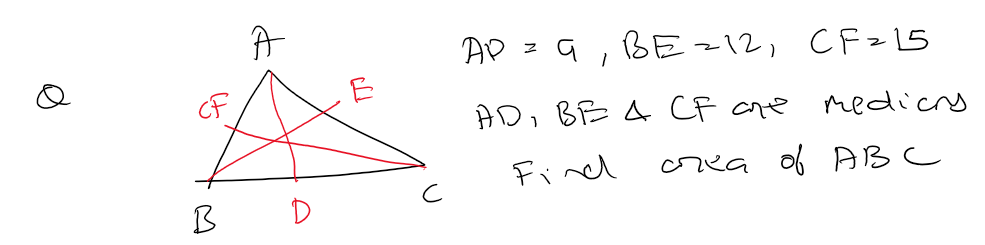
\includegraphics[width=0.7\linewidth]{Quant//Geometry//Images//Triangles/area_of_triangle_question_1.png}
\end{figure*}

We will arrange the medians in a triangle and apply the above theorem. First, let us see which sides of triangle satisfy the pythagoreas theorem or not
\begin{align*}
    15^2 = 9^2 + 12^2
\end{align*}

Based on this, this is how the triangle will look like
\begin{figure*}[h!]
    \centering
    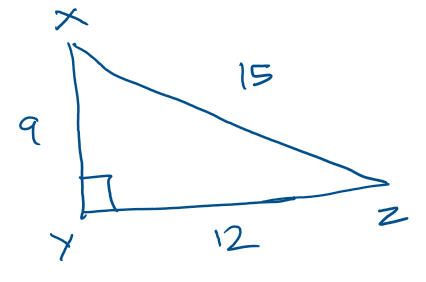
\includegraphics[width=0.5\linewidth]{Quant//Geometry//Images//Triangles/area_of_triangle_question_1_solution.png}
\end{figure*}

\begin{itemize}
    \item Area ($\Delta XYZ$) = $\dfrac{1}{2} * 9 * 12 = 54$. 
    \item Area ($\Delta ABC$) = $\dfrac{3}{4} * 54 = 72$. 
\end{itemize}

\SampleQuestion{Find AD in the following figure}

\begin{figure*}[h!]
    \centering
    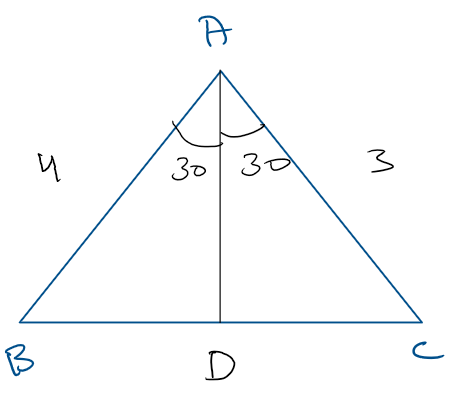
\includegraphics[width=0.40\linewidth]{Quant//Geometry//Images//Triangles/area_of_triangle_question_2.png}
\end{figure*}

Area of ABC 
\begin{itemize}
    \item Using trigonometry : $\dfrac{1}{2} * 4 * 3 * \sin{60} = 3 \sqrt{3}$
    \item In terms of smaller triangles : $\Area{ABC} = \Area{ABD} + \Area{ACD}$
\end{itemize}

\begin{align*}
    \Area{ABC} &= \bigParen{\dfrac{1}{2} * 4 * AD * \sin{30}} +  \bigParen{\dfrac{1}{2} * 3 * AD * \sin{30}} \\
    3 \sqrt{3} &= \dfrac{1}{4} * \bigParen{4 * AD + 3 * AD} \tag{$\sin{30} = \frac{1}{2} $} \\
    12 \sqrt{3} &= 7 * AD \\
    AD &= \dfrac{12 \sqrt{3}}{7}
\end{align*}

\SampleQuestion{A semicircle is inside a triangle with its origin on the side $BC$ as shown below .Find the radius $r$ of the semicircle}

\begin{figure*}[h!]
    \centering
    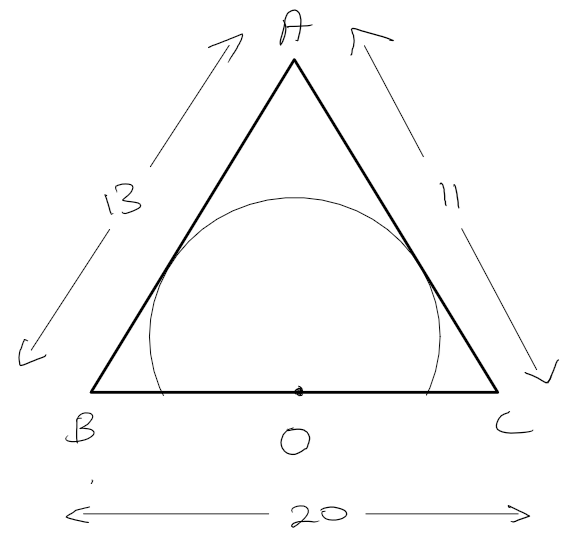
\includegraphics[width=0.4\linewidth]{Quant//Geometry//Images//Triangles/area_of_triangle_question_3.png}
\end{figure*}

We need to find $r$ as shown in the above figure. To do so, we can equate area of $\Triangle ABC$ with area of triangles $\Triangle AOB$ and $\Triangle AOC$. We can see that $ \Area{ABC} = \Area{AOB} + \Area{AOC} $

\begin{figure*}[h!]
    \centering
    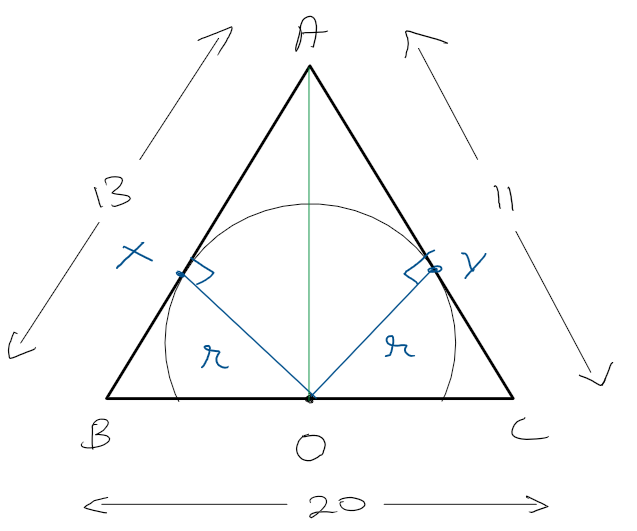
\includegraphics[width=0.5\linewidth]{Quant//Geometry//Images//Triangles/area_of_triangle_question_4_sol_fig.png}
\end{figure*}

\textbf{Calculating $\Area{ABC}$}
$s = \dfrac{13 + 11 + 20}{2} = 22$

\begin{align*}
    \Area{ABC} &= \sqrt{s * (s - a) * (s - b) * (s - c)} \\
    &= \sqrt{22 * (22 - 13) * (22 - 20) * (22 - 11)} \\
    &= \sqrt{22 * 9 * 2 * 11} \\
    &= \sqrt{2 * 11 * 3 * 3 * 2 * 11} \\
    &= 66
\end{align*}

\textbf{Calculating $\Area{ABO}$}
Base = 13, Height = $OB = r$
\begin{align*}
    \Area{ABO} &= \dfrac{1}{2} * 13 * r
\end{align*}

\textbf{Calculating $\Area{ACO}$}
Base = 11, Height = $OC = r$
\begin{align*}
    \Area{ABO} &= \dfrac{1}{2} * 11 * r
\end{align*}

\textbf{Equating Areas}
\begin{align*}
    \Area{ABC} &= \Area{AOB} + \Area{AOC} \\
    66 &= \dfrac{1}{2} * (13r + 11r) \\
    r &= \dfrac{2 * 66}{24} \\
    r &= 5.5
\end{align*}

\SampleQuestion{In $\Triangle ABC$, $AB = 17.5, AC = 9.$ Let $D$ be a point on BC such that AD is perpendicular to BC. If $AD = 3$ then what is the radius of the circle circumscribing $\Triangle ABC$ ?}

\begin{figure*}[h!]
    \centering
    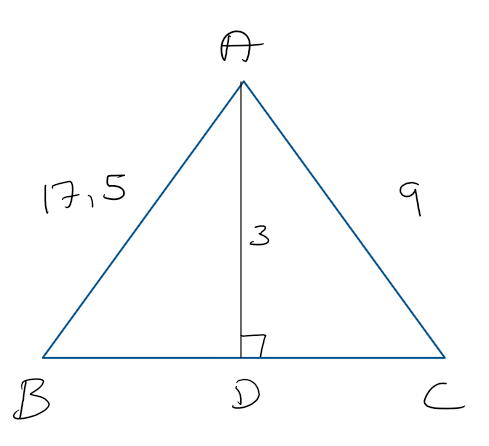
\includegraphics[width=0.4\linewidth]{Quant//Geometry//Images//Triangles/geo_center_question_2.png}
\end{figure*}

\begin{itemize}
    \item Area of triangle using Circumradius = $\dfrac{AB * AC * BC}{4 * R}$
    \item Area of triangle using base and height = $\dfrac{1}{2} * BC *  AD$
\end{itemize}

Using the above 
\begin{align*}
    \dfrac{AB * AC * BC}{4 * R} &= \dfrac{1}{2} * BC *  AD \\
    R &= \dfrac{AB * AC * BC * 2}{4 * BC * AD} \\
    &= \dfrac{17.5 * 9 * 2}{4 * 3} \tag{Removed BC as it is common} \\
    &= 26.25
\end{align*}







\newpage
\section{Angle Bisector Theorem}
An angle bisector divides the base in the ratio of the other sides of triangle. This is true for both internal and external angle bisectors

\begin{figure*}[h!]
    \centering
    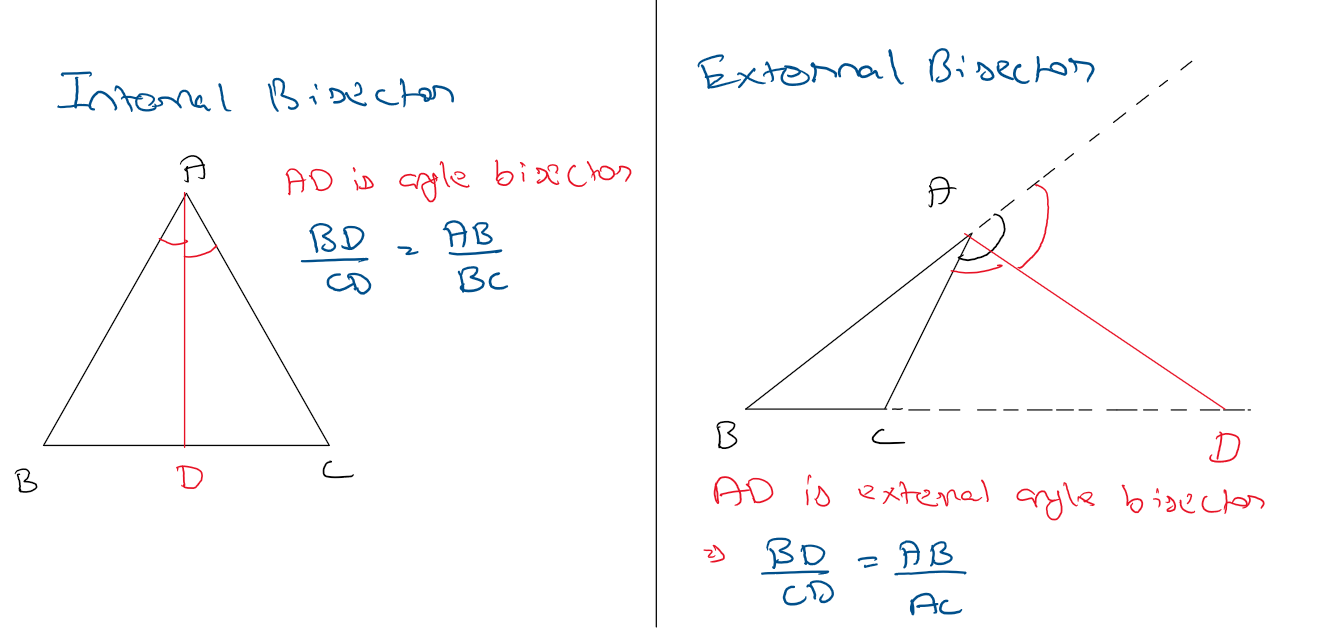
\includegraphics[width=1.02\linewidth]{Quant//Geometry//Images//Triangles/angle_bisector_theorem.png}
\end{figure*}

In the external angle bisector case, we "extended" $BC$ and determined a point $D$ at which $AD$ will divide the exterior $\angle A$ in two equal parts. The partitions created by point $D$ are still $BD$ and $CD$ (even though visually, it looks like $C$ divides $BD$)





























\newpage

\section{Right Triangles}
\subsection{Orthocenter and Circumcenter}
A right triangle is a triangle where one side has right angle. 

\begin{figure*}[h!]
    \centering
    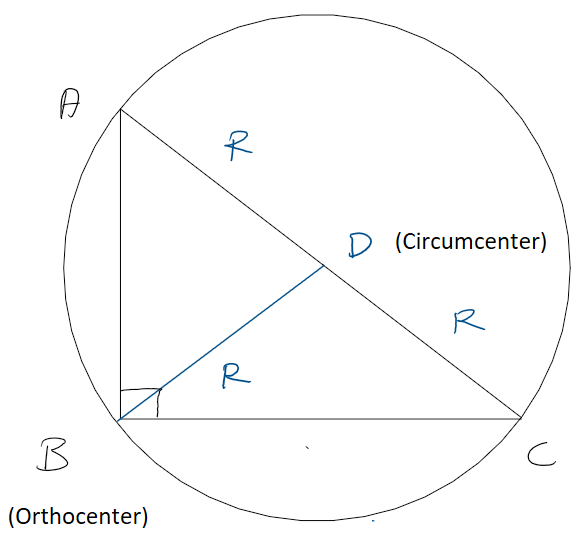
\includegraphics[width=0.5\linewidth]{Quant//Geometry//Images//Triangles/rt_triangle_ortho_circumcenter.png}
\end{figure*}

In the figure above, there are few interesting properties about right triangle
\begin{itemize}
    \item Circumcenter is midpoint of hypotenuse (Point $D$)
    \item Orthocenter is the vertex where the $\degree{90}$ is present (Point $B$)
    \item The line joining orthocenter and circumcenter is median of triangle with the length $R = $ circumradius. ($BD = AD = CD$)
    \item Circumradius of triangle is $\dfrac{1}{2} * \text{ hypotenuse } $ ($\dfrac{AC}{2}$)
\end{itemize}

\newpage

\subsection{Incircle in terms of Hypotenuse}
Before we explore this, we should know this property of circles : \textbf{Two tangents drawn from same point to a circle are equal}. In the below figure, from $P$ we have drawn two tangents $PA$ and $PB$ to circle. According to above property, $PA = PB$

\begin{figure*}[h!]
    \centering
    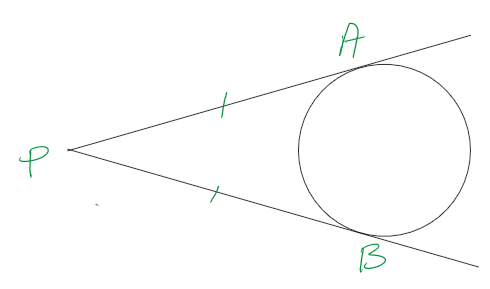
\includegraphics[width=0.4\linewidth]{Quant//Geometry//Images//Triangles/two_tangents_from_same_pt_circle.png}
\end{figure*}

Using this, we can prove that Inradius $r$ of a right triangle is given as 

\begin{align*}
    r &= s - h \tag{$ s = \dfrac{a + b + c}{2} $} \\
    \tag{$h = \text{hypotenuse}$}
\end{align*}

Let us try to derive this. Let us refer the example below. In the below figure, we have $\Triangle ABC$ where the circle inscribed inside the triangle has its origin on incenter. Therefore, $r$ represents inradius.

\begin{figure*}[h!]
    \centering
    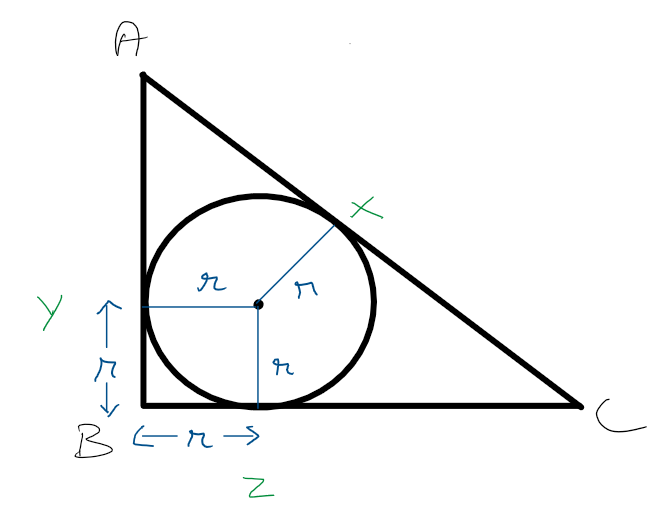
\includegraphics[width=0.5\linewidth]{Quant//Geometry//Images//Triangles/rt_triangle_inradius_hypo_theory.png}
\end{figure*}

In this triangle, $AB = c, BC = a, AC = b$. Using the property we discussed above for circles and tangents, we can say the following things
\begin{itemize}
    \item  $CZ = a - r, CX = a - r$ (Tangent from point $C$)
    \item  $AY = c - r, AX = c - r$ (Tangent from point $A$)
\end{itemize}

Hypotenuse is defined by $b$. We can see that
\begin{align*}
    b &= (a - r) + (c - r) \\
    2r &= a + c - b \\
    r &= \dfrac{a + c - b}{2} \\
    r &= \dfrac{a + b + c}{2} - b \tag{If you solve this, it will give the original expression back} \\
    r &= s - h \tag{$s = \dfrac{a + b + c}{2}, h = $ hypotenuse}
\end{align*}

\subsection{Pythagorean Triplets}
A group of 3 numbers which satisfies the pythagorean theorem. Some of the basic triplets are as follows (\textbf{memorise them})
\begin{enumerate}
    \item 3,4,5 ($5^2 = 3^2 + 4^2$)
    \item 5,12,13 ($13^2 = 5^2 + 12^2$)
    \item 7,24,25 ($25^2 = 7^2 + 24^2$)
    \item 8,15,17 ($17^2 = 8^2 + 15^2$)
    \item 9,40,41 ($41^2 = 9^2 + 40^2$)
    \item 20,21,29 ($29^2 = 20^2 + 21^2$)
\end{enumerate}

\SampleQuestion{Can we create a right triangle with sides of length 18,24,30 ?}

$18,24,30 = 6 * 3, 6 * 4, 6 * 5$. Taking 6 common, we will have $(3,4,5)$. Since this is a multiple of the basic pythagorean triplet we listed above, we can create a right triangle with these dimensions

\SampleQuestion{Find area of triangle with sides of length 15, 36, 39}

$15, 36, 39 = 3 * 5, 3 * 12, 3 * 13$. Taking 3 common, we will have $(5,12,13)$. Since this is a multiple of the basic pythagorean triplet we listed above, we can create a right triangle with these dimensions. The right triangle will have 
\begin{itemize}
    \item Base = 12
    \item Height = 5
    \item Hypotenuse = 13
\end{itemize}

Area = $\dfrac{1}{2} * 5 * 12 = 30$. Now, area of original triangle = $9 * 30 = 270$. We multiply with 9 (instead of 3) because area of triangle is defined as $\dfrac{1}{2} * b * p$. Now, in this question, $b = 3 * 5, p = 3 * 12$. We can see that the constant $3$ is multiplied twice

\subsection{Formation of pythagorean triplets}
Let us assume we have three numbers $(a,b,c)$. To form a pythagorean triplet, we have the following conditions

\subsubsection{Odd Values}
\begin{itemize}
    \item $\dfrac{b + c}{2} = \dfrac{a^2}{2}$
    \item $b$ and $c$ will be consecutive numbers
\end{itemize}

\begin{table}[h!]
    \centering
    \begin{tabular}{|| c | c | c | c ||}
        \hline
         \textbf{Triplet} & \textbf{a} & $\dfrac{a^2}{2}$ & $\dfrac{b + c}{2}$  \\
        \hline
         (3,4,5) & 3 & 4.5 & $\dfrac{4 + 5}{2} = 4.5 $ \\
        \hline
         (5,12,13) & 5 & 12.5 & $\dfrac{12 + 13}{2} = 12.5 $ \\
        \hline
         (11,60,61) & 5 & 60.5 & $\dfrac{60 + 61}{2} = 60.5 $ \\
        \hline
         (11,60,61) & 5 & 60.5 & $\dfrac{60 + 61}{2} = 60.5 $ \\
        \hline
    \end{tabular}
\end{table}

\subsubsection{Even Values}
\begin{itemize}
    \item $\dfrac{b + c}{2} = \dfrac{a^2}{4}$
    \item $b$ and $c$ will have difference of 2
\end{itemize}

\begin{table}[h!]
    \centering
    \begin{tabular}{|| c | c | c | c ||}
        \hline
         \textbf{Triplet} & \textbf{a} & $\frac{a^2}{4}$ & $\frac{b + c}{2}$  \\
        \hline
         (4,3,5) & 4 & 4 & $\dfrac{3 + 5}{2} = 4 $ \\
        \hline
         (8,15,17) & 8 & 16 & $\dfrac{15 + 17}{2} = 16 $ \\
        \hline
         (12,35,37) & 12 & 36 & $\dfrac{35 + 37}{2} = 36 $ \\
        \hline
    \end{tabular}
\end{table}

\SampleQuestion{Find sum of inradius of $\Triangle{ABD}$ and $\Triangle{ADC}$}

\begin{figure*}[h!]
    \centering
    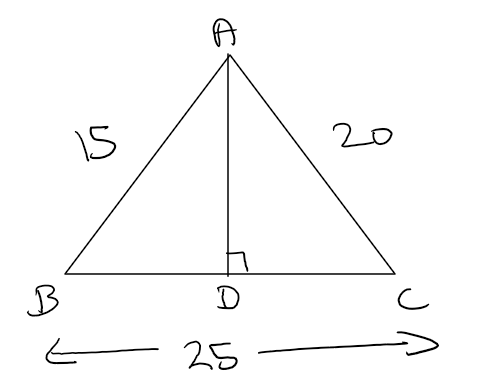
\includegraphics[width=0.4\linewidth]{Quant//Geometry//Images//Triangles/rodha_triangle_5_q1.png}
\end{figure*}

In a right triangle, inradius is defined as difference of $s$ and $h$ where $s = \dfrac{a + b + c}{2}$ and $h = \text{hypotenuse}$. To calculate inradius for the two triangles, we need to find $AD$ and the bases of their triangles

\vspace{1cm}

\textbf{Finding AD}
\begin{itemize}
    \item We will calculate area of ABC and then use $\dfrac{1}{2} * \text{base} * \text{height}$ formula where base = BC, height = AD
    
    \item $s = \dfrac{a + b + c}{2} \implies \dfrac{15 + 20 + 25}{2} = 30$

    \item $\Area{ABC} = \sqrt{30 * (30 - 15) * (30 - 20) * (30 - 25)} \implies \sqrt{30 * 15 * 20 * 25} = 150$

    \item Using base and height, $\Area{ABC} = \dfrac{1}{2} * 25 * AD \implies 150 = \dfrac{1}{2} * 25 * AD \implies AD = 12$
\end{itemize}

\vspace{1cm}

$\Triangle{ABD}$ \\
Using pythagoreas theorem, we can find value of $BD$ 
\begin{align*}
    AB^2 &= AD^2 + BD^2 \\ 
    BD &= \sqrt{AB^2 - AD^2} \\
    &= \sqrt{15^2 - 12^2} \\
    &= \sqrt{27 * 3} \\
    &= 9
\end{align*}

Inradius of $\Triangle{ABD}$
\begin{align*}
    r_{ABD} &= s_{ABD} - h_{ABD} \\
    &= \dfrac{15 + 12 + 9}{2} - 15 \\
    &= 18 - 15 = 3
\end{align*}

\vspace{1cm}

$\Triangle{ADC}$ \\
We know that $BD = 9 \implies DC = 16$. We can find $r_{ABD}$ as 
\begin{align*}
    r_{ABD} &= s_{ABD} - h_{ABD} \\
    &= \dfrac{20 + 16 + 12}{2} - 20 \\
    &= 24 - 20 = 4
\end{align*}

\textbf{Sum of inradius = } 7


\newpage

\SampleQuestion{ABCD is a rectangle with DC = 12 and BC = 9. Find the distance between incenters of $\Triangle{ADC}$ and $\Triangle{ABC}$}

\begin{figure*}[h!]
    \centering
    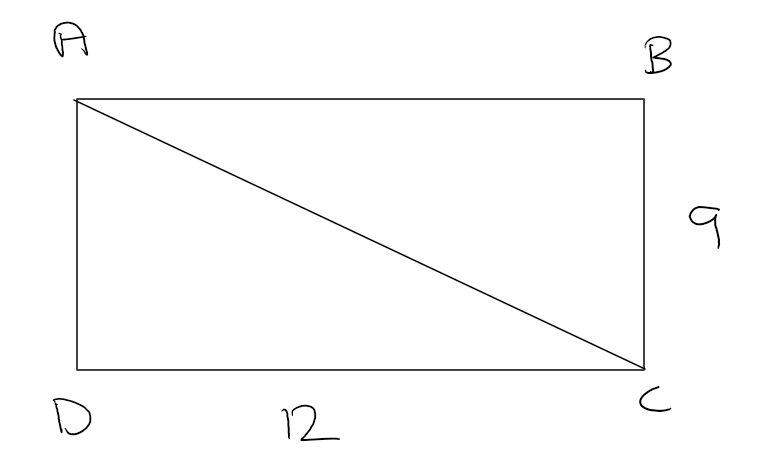
\includegraphics[width=0.5\linewidth]{Quant//Geometry//Images//Triangles/rodha_triangle_5_q2_1.png}
\end{figure*}

In the rectangle, $\angle{D} = \angle{B} = \degree{90}$. We can find AC as $AC^2 = AD^2 + DC^2 \implies AC = 15$. Using the formula $r = s - h$ to find inradius, we can find inradius of both triangles as follows
\begin{itemize}
    \item For both triangles, $s = \dfrac{12 + 15 + 9}{2} = 18$
    \item $\Triangle{ADC}$ : 18 - 15 = 3
    \item $\Triangle{ABC}$ : 18 - 15 = 3
\end{itemize}

Now, look at the diagram below. We see that we can form a triangle where $r_1 \text{and} r_2$ are the hypotenuse of a triangle with base = 6 and height = 3 (triangle created by red color). 

\begin{figure*}[h!]
    \centering
    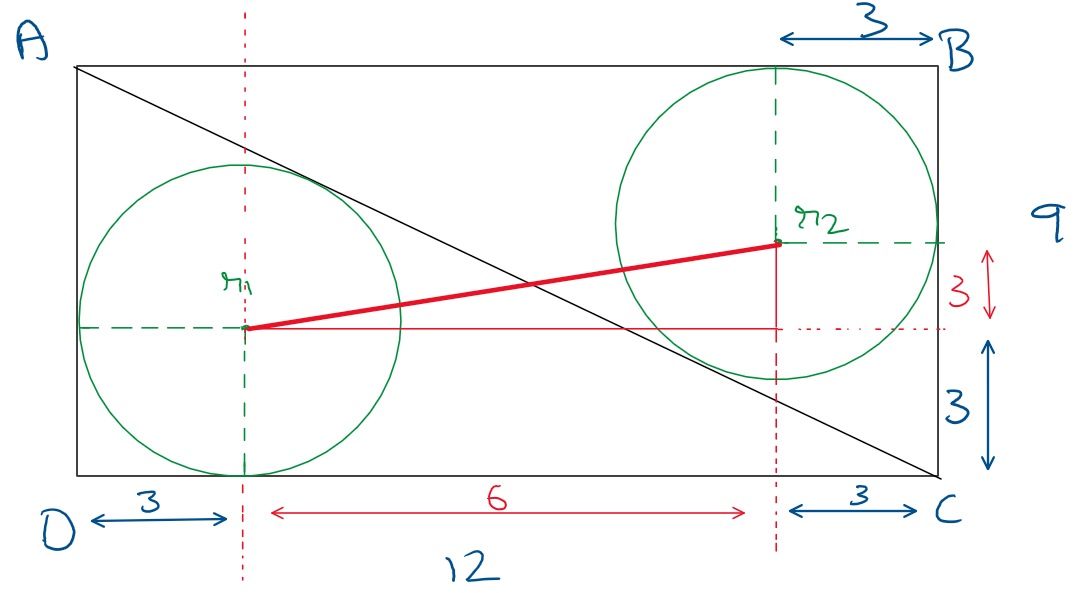
\includegraphics[width=0.7\linewidth]{Quant//Geometry//Images//Triangles/rodha_triangle_5_q2_2.png}
\end{figure*}

Distance between incenters = $\sqrt{6^2 + 3^2} \implies \sqrt{45} = 3 \sqrt{5}$

\newpage

\SampleQuestion{In a right triangle, area = 80 and perimeter = 80. Find the length of the hypotenuse}

We can write the area of a triangle in terms of its perimeter (semiperimeter $s$) as $r * s$ where $r = \text{Inradius}$. In a right triangle, $r = s - h$ where $h = \text{hypotenuse}$. Using these, we can find our values
\begin{itemize}
    \item $s = \dfrac{p}{2} \implies \dfrac{80}{2} = 40$
    \item Finding $r$ through area : $80 = r * 40 \implies r = 2$
    \item Finding $h$ through $r$ : $r = s - h \implies h = s - r \implies h = 38$
\end{itemize}

\SampleQuestion{What is the area of a right triangle with R (circumradius) = 18 and r (inradius) = 8 ?}

\begin{itemize}
    \item In a right triangle, $R = \frac{h}{2}$ where $h = hypotenuse$. From above, we can get $h = 36$

    \item In a right triangle, $r = s - h \implies s = 8 + 36 = 44$

    \item Area = $r * s = 8 * 44 = 352$
\end{itemize}

\SampleQuestion{In a right triangle, $a,b,c$ are sides of traingles where $c > b > a$. Also, we are given that $a = 12$ and $2a + 7c = 9b$. Find the value of $c$}

\textbf{THIS IS A MIND BOGGLING QUESTION. TRY TO UNDERSTAND THE APPROACH BECAUSE IT IS NOT INTUITIVE}

We will be using the concept of pythagorean triplets in this one. Let us the equation to arrive at an interesting result

\begin{align*}
    2a + 7c &= 9b \\
    2a + 7c &= 2b + 7b \\
    2 * (a - b) &= 7 * (b - c) \\
    \dfrac{a - b}{b - c} &= \dfrac{7}{2}
\end{align*}

We came to a ratio where $a - b = 7$ and $b - c = 2$. Let us do hit and trial on the common pythagorean triplets
\begin{itemize}
    \item 3,4,5 : 4-3 = 1 REJECTED
    \item 5,12,13 : 12 - 5 = 7, 13 - 12 = 1 REJECTED
    \item 7,24,25 : 24 - 7 = 17 REJECTED
    \item 8,15,17 : 15 - 8 = 7, 17 - 15 = 2 ACCEPTED
\end{itemize}

Now, our first term of triplet is 12. To be of the form 8,15,17, we need to find the coefficient $\implies k = \dfrac{12}{8} = 1.5$. The triplet is, therefore $(12, 1.5 * 15, 1.5 * 17) = (12,22.5,25.5)$








\newpage

\section{Similarity of Triangles}

\hl{(WRITING THE THEORY PART ONLY. MAKE DIAGRAMS AND OTHER STUFF ON WEEKDAYS ALSO, FINISH ABOVE FIRST)}

Similarity is between two triangles. When two triangles are similar, we have the following properties
\begin{itemize}
    \item Ratio of corresponding sides are equal
    \item Ratio of corresponding sides = Ratio of Heights = Ratio of medians = Ratio of inradius = Ratio of circumradius
    \item Ratio of area = square of ratio of heights
\end{itemize}





\subsection{Types of similarity}

\subsubsection{SSS : Side, Side, Side}
Sides of two triangles are in same ratio. $\dfrac{AB}{PQ} = \dfrac{BC}{QR} = \dfrac{AC}{PR}$


\begin{figure*}[h!]
    \centering
    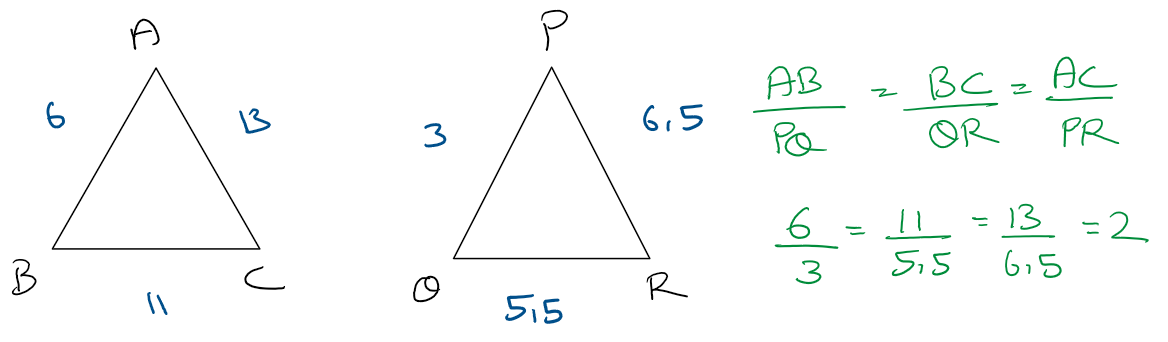
\includegraphics[width=0.8\linewidth]{Quant//Geometry//Images//Triangles/rodha_triangle_6_sss.png}
\end{figure*}

\subsubsection{AA : Angle, Angle}
Two angles . $\angle ADE = \angle ABC, \angle AED = \angle ACB$

\begin{figure*}[h!]
    \centering
    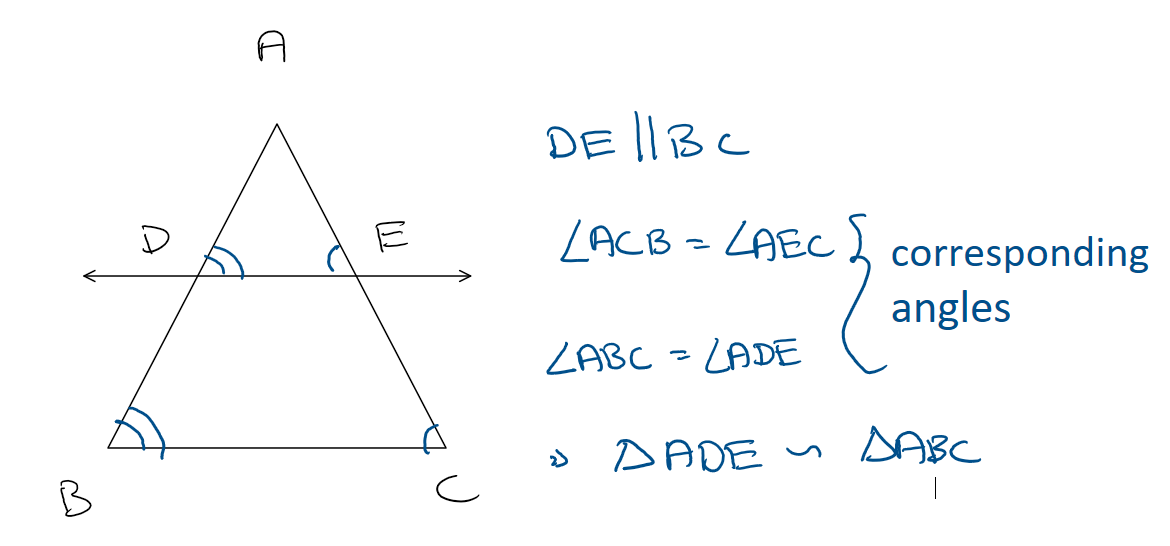
\includegraphics[width=0.9\linewidth]{Quant//Geometry//Images//Triangles/rodha_triangle_6_aa.png}
\end{figure*}

\subsubsection{SAS : Side, Angle, Side}

\begin{figure}[h!]
    \centering
    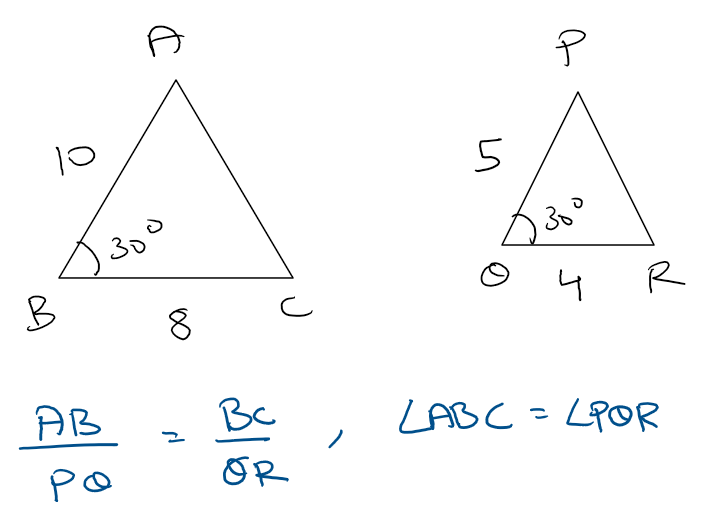
\includegraphics[width=0.5\linewidth]{Quant//Geometry//Images//Triangles/rodha_triangle_6_sas.png}
\end{figure}

\textbf{The angle must be between the two sides}. Ratio of two sides and the included angle is equal. $\dfrac{AB}{PQ} = \dfrac{BC}{QR}, \angle ABC = \angle PQR$. In this, $\angle ABC$ and $\angle PQR$ lie between AB and PQ respectively





\subsection{Determining How to find the sides / angles which should be similar}

Let us explore this using two cases

\subsubsection{CASE 1}

Let us say that we are given the following triangle and we need to find whether $\Triangle{ABC}$ is similar to $\Triangle{AXY}$ or not. In this triangle, XYZW is a rectangle that is inscribed inside the triangle

\begin{figure}[h!]
    \centering
    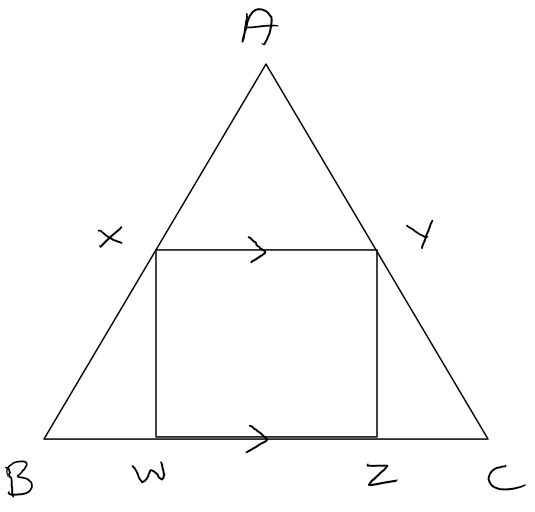
\includegraphics[width=0.5\linewidth]{Quant//Geometry//Images//Triangles/rodha_triangle_6_similarity_equation_case_1.png}
\end{figure}

We know that sides of a rectangle are parallel to each other. Using this, we can make some relations between the angles. In the below figure, we have marked $\angle{ABC} \text{ and } \angle{ACB} \text{ as } \theta \text{ and } \phi$ respectively. Using corresponding angles, $\angle{AXY} = \angle{ABC}$ and $\angle{AYX} = \angle{ACB}$. 

\begin{figure}
    \centering
    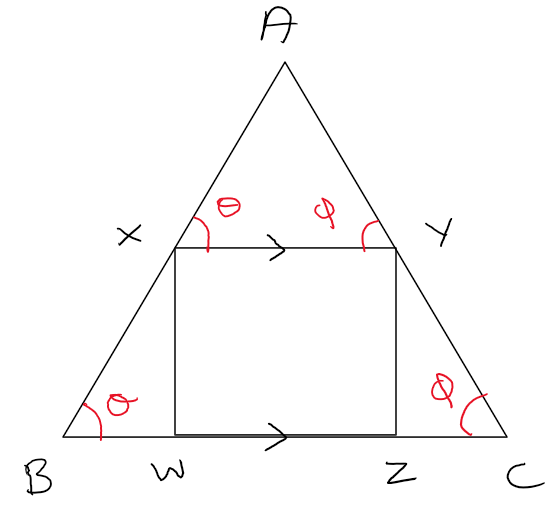
\includegraphics[width=0.5\linewidth]{Quant//Geometry//Images//Triangles/rodha_triangle_6_similarity_equation_case_1_2.png}
\end{figure}

We can now check for similarity between $\Triangle{AXY} \text{and} \Triangle{ABC}$
\begin{itemize}
    \item $\angle{AXY} = \angle{ABC}$
    \item $\angle{AYX} = \angle{ACB}$
    \item Hence proved similar through AA condition
\end{itemize}

To write the ratio of the sides, we will take the help of angles
\begin{table}[h!]
    \centering
    \begin{tabular}{|| c | c | c | c | c ||}
        \hline
         Angle in $\Triangle{AXY}$ & Side & Angle in $\Triangle{ABC}$ & Side & Ratio  \\
        \hline
         $\angle{AXY}$ & AY & $\angle{ABC}$ & AC & $\dfrac{AY}{AC}$ \\ 
         \hline
         $\angle{AYX}$ & AX & $\angle{ACB}$ & AB & $\dfrac{AX}{AB}$ \\ 
         \hline
         $\angle{XAY}$ & XY & $\angle{BAC}$ & BC & $\dfrac{XY}{BC}$ \\ 
         \hline
    \end{tabular}
\end{table}

\begin{NOTE}
    An interesting observation is in the notation of how we right angles. When we write an angle, say $\angle{ABC}$, $B$ is the part where the angle "exists" and $A$ and $C$ are the points that make that angle possible. In $\Triangle{ABC}$ , $\angle{ABC}$ is formed through the edge $AC$. This is a useful observation in writing similarity ratios
\end{NOTE}

\subsubsection{CASE 2}

This is an interesting case where we have a right triangle as follows

\begin{figure}[h!]
    \centering
    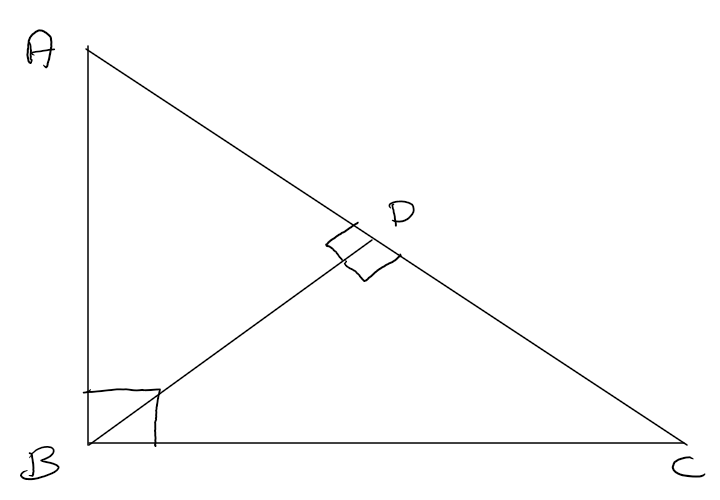
\includegraphics[width=0.5\linewidth]{Quant//Geometry//Images//Triangles/rodha_triangle_6_similarity_equation_case_2.png}
\end{figure}

In this triangle, we need to find whether the following triangles are similar or not

\begin{itemize}
    \item $\Triangle{ABD}$ and $\Triangle{CBD}$
    \item $\Triangle{ABC}$ and $\Triangle{ABD}$
    \item $\Triangle{ABC}$ and $\Triangle{CBD}$
\end{itemize}

\textbf{ First, let's start with $\Triangle{ABD}$ and $\Triangle{CBD}$ }

Let us assume that $\angle{ACB} = \theta$

In $\Triangle{BCD}$
\begin{align*}
    \angle{DBC} + \angle{BDC} + \angle{DCB} &= \degree{180} \tag{Angle sum property of triangle} \\
    \angle{DBC} + 90 + \theta &= \degree{180} \\
    \angle{DBC} &= 90 - \theta
\end{align*}

Now, we can see that $\angle{ABC} = \angle{ABD} + \angle{DBC} = \degree{90} \implies \angle{ABD} = \theta$

In $\Triangle{ABD}$
\begin{align*}
    \angle{BAD} + \angle{ADB} + \angle{DBA} &= \degree{180} \tag{Angle sum property of triangle} \\
    \angle{BAD} + 90 + \theta &= \degree{180} \\
    \angle{BAD} &= 90 - \theta
\end{align*}

We get a figure like this in the end

\begin{figure}[h!]
    \centering
    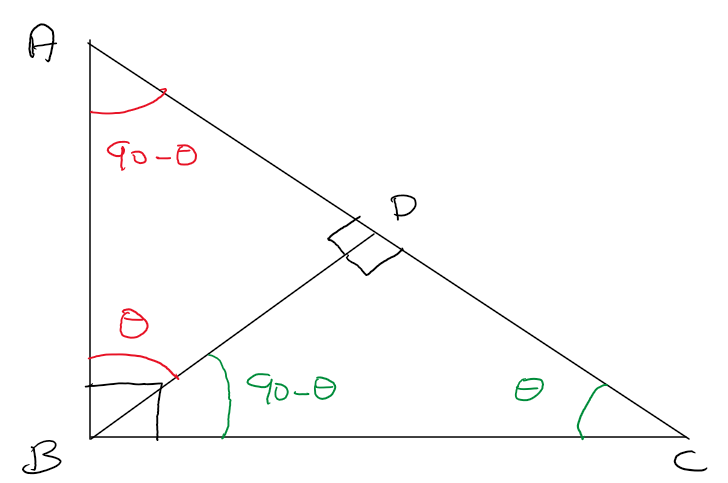
\includegraphics[width=0.5\linewidth]{Quant//Geometry//Images//Triangles/rodha_triangle_6_similarity_equation_case_2_2.png}
\end{figure}

We can find simlarity between $\Triangle{ABD}$ and $\Triangle{CBD}$ as follows
\begin{itemize}
    \item $\angle{DCB} = \angle{DBA}$
    \item $\angle{DBC} = \angle{DAB}$
    \item Hence similar by AA condition
\end{itemize}

To write the ratio of the sides, we will take the help of angles
\begin{table}[h!]
    \centering
    \begin{tabular}{|| c | c | c | c | c ||}
        \hline
         Angle in $\Triangle{ADB}$ & Side & Angle in $\Triangle{BDC}$ & Side & Ratio  \\
        \hline
         $\angle{BAD}$ & BD & $\angle{DBC}$ & DC & $\dfrac{BD}{DC}$ \\ 
         \hline
         $\angle{ABD}$ & AD & $\angle{DCB}$ & DB & $\dfrac{AD}{DB}$ \\ 
         \hline
         $\angle{ADB}$ & AB & $\angle{BDC}$ & BC & $\dfrac{AB}{BC}$ \\ 
         \hline
    \end{tabular}
\end{table}

\textbf{ Now, with $\Triangle{ABC}$}
\begin{itemize}
    \item $\Triangle{ABD}$
    \begin{itemize}
        \item $\angle{BAD} = \angle{CAB}$
        \item $\angle{ABD} = \angle{ACB}$
        \item Hence similar by AA
        \item Ratio = $\dfrac{BD}{CB} = \dfrac{AD}{AB} = \dfrac{AB}{AC}$
    \end{itemize}

    \item $\Triangle{BDC}$
    \begin{itemize}
        \item $\angle{DBC} = \angle{CAB}$
        \item $\angle{DCB} = \angle{ACB}$
        \item Hence similar by AA
        \item Ratio = $\dfrac{DC}{CB} = \dfrac{DB}{AB} = \dfrac{BC}{AC}$
    \end{itemize}
\end{itemize}

\SampleQuestion{A square PQRS of length $x$ is inscribed a triangle ABC as shown in the figure below. Find the length of square}

\begin{figure}[h!]
    \centering
    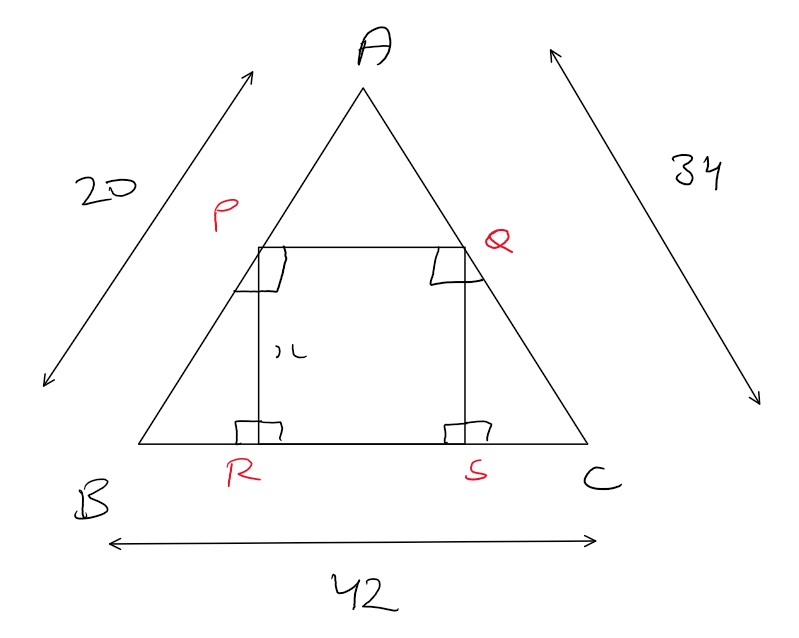
\includegraphics[width=0.5\linewidth]{Quant//Geometry//Images//Triangles/rodha_triangle_6_question_1.png}
\end{figure}

In a square, the sides are parallel to each other. We can use that property to make $\Triangle{APQ}$ similar to $\Triangle{ABC}$ as $\angle{APQ} = \angle{ABC} \text{and} \angle{AQP} = \angle{ACB}$ because they are corresponding angles respectively. Since these two angles are equal, $\Triangle{APQ}$ is similar to $\Triangle{ABC}$ through the AA similarity condition \\

To find the length of the square, we can draw a perpendicular AY intersecting PQ at point X. Since it is a perpendicular, the length of segment XY is equal to the side of square. \textbf{We can use the three sides of $\Triangle{ABC}$ to find $AY$ and compare ratio of sides with heights}

\begin{figure}[h!]
    \centering
    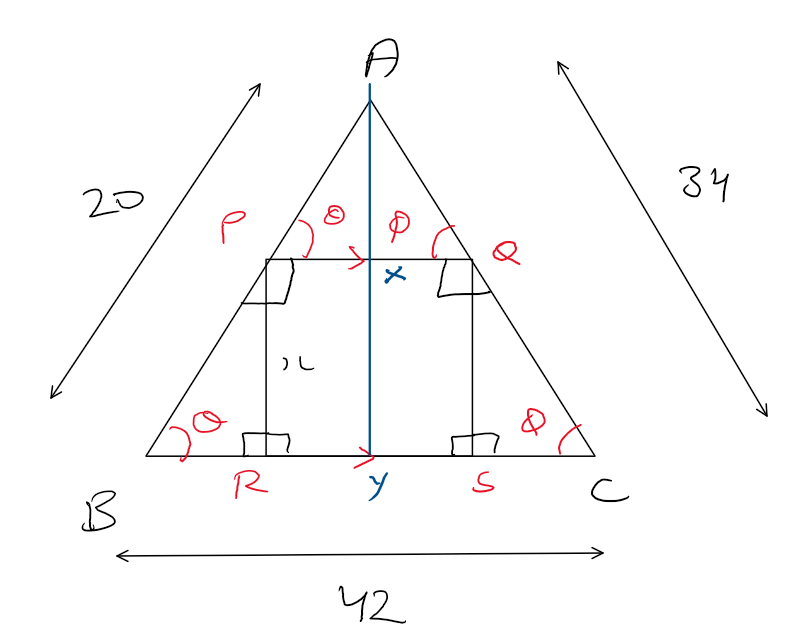
\includegraphics[width=0.5\linewidth]{Quant//Geometry//Images//Triangles/rodha_triangle_6_question_1_1.png}
\end{figure}

We can use the concept of pythagorean triplets to find the height $AY$. Let us take $\Triangle{AYC}$ where hypotenuse = $AC = 34$. Let us compare with a few common triplets. We can write $34 = 2 * 17$. \textit{While we can use any triplet to find a coefficient such that hypotenuse = 34 and triplet satisfies pythagorean theorem, for sake of easy calculation, let us keep to integer and simple values only}
\begin{itemize}
    \item 3,4,5 
    \item 5,12,13,
    \item 6,8,10
    \item 7,24,25
    \item 8,15,17 ... We can use this as it contains 17
\end{itemize}

We know that $34 = 2 * 17$. Therefore, for our triplet, our coefficient is 2 $\implies$ dimensions are 16,30 and 34. By observing our figure, we can say that $YC = 30$ and $AY = 16$. Now, let's use the similarity conditions between $\Triangle{APQ}$ and $\Triangle{ABC}$

\begin{align*}
    \dfrac{PQ}{BC} &= \dfrac{AX}{AY} \\
    \dfrac{x}{42} &= \dfrac{16 - x}{16} \tag{AX = AY - XY} \\
    16x &= 42 * 16 - 42x \\
    x &= \dfrac{42 * 16}{58} \\
    &= \dfrac{336}{29}
\end{align*}

\textbf{Note : Triangles 8 should be seen before Triangles 7}

\newpage


















\section{Conditions for Formation of Triangle}

\subsection{General Formula}
For a triangle, the relation of sides is as follows : Difference of two sides $<$ third side $<$ Sum of two sides. Refer to the following questions

\SampleQuestion{If sides of triangle are $(7,12,n)$, for how many integral values of $n$ the triangle will be formed?}

The third side $n$ is related to other sides $(7,12)$ as $12 - 7 < n < 12 + 7 \implies 5 < n < 19$. The number of values of $n$ is $19 - 5 - 1 = 13$

\SampleQuestion{If 2 sides of a triangle 762 and 1233 units. For how many integral values of 3rd side, a triangle will be formed}

The third side is related to other sides as : $1233 - 762 < \text{third side} < 1233 + 762 \implies 501 < \text{third side} < 1965$. The number of integral values is $1965 - 501 - 1 = 1523$

\subsection{Condition for right, obtuse and acute triangles}
We can use the pythagoreas theorem to deduce conditions through which we can determine whether a triangle is a right, obtuse or acute triangle. It is summarised in the below table for $\Triangle{ABC}$. The sides are marked as follows : $AC = c, BC = b, AB = a$. In the table below, \textbf{the side $c$ is assumed to be the largest}

\begin{table}[h!]
    \centering
    \begin{tabular}{|| c | c ||}
        \hline
         $\angle{ABC}$ & Condition  \\
        \hline
         $= \degree{90}$ & $c^2 = a^2 + b^2$ \\ 
        \hline
         $> \degree{90}$ & $c^2 > a^2 + b^2$ \\ 
        \hline
         $< \degree{90}$ & $c^2 < a^2 + b^2$ \\ 
        \hline
    \end{tabular}
\end{table}

To make sense of this, imagine a right triangle $ABC$ where $\angle{ABC} = \degree{90}$. If we increase the angle, we can see that the side $AC$ increases in response. Similarly, if we decrease the angle, the side decreases in response. This is because of a principle (more like an observation) : \textbf{Larger the angle, larger the side opposite to that angle}

\begin{figure}[h!]
    \centering
    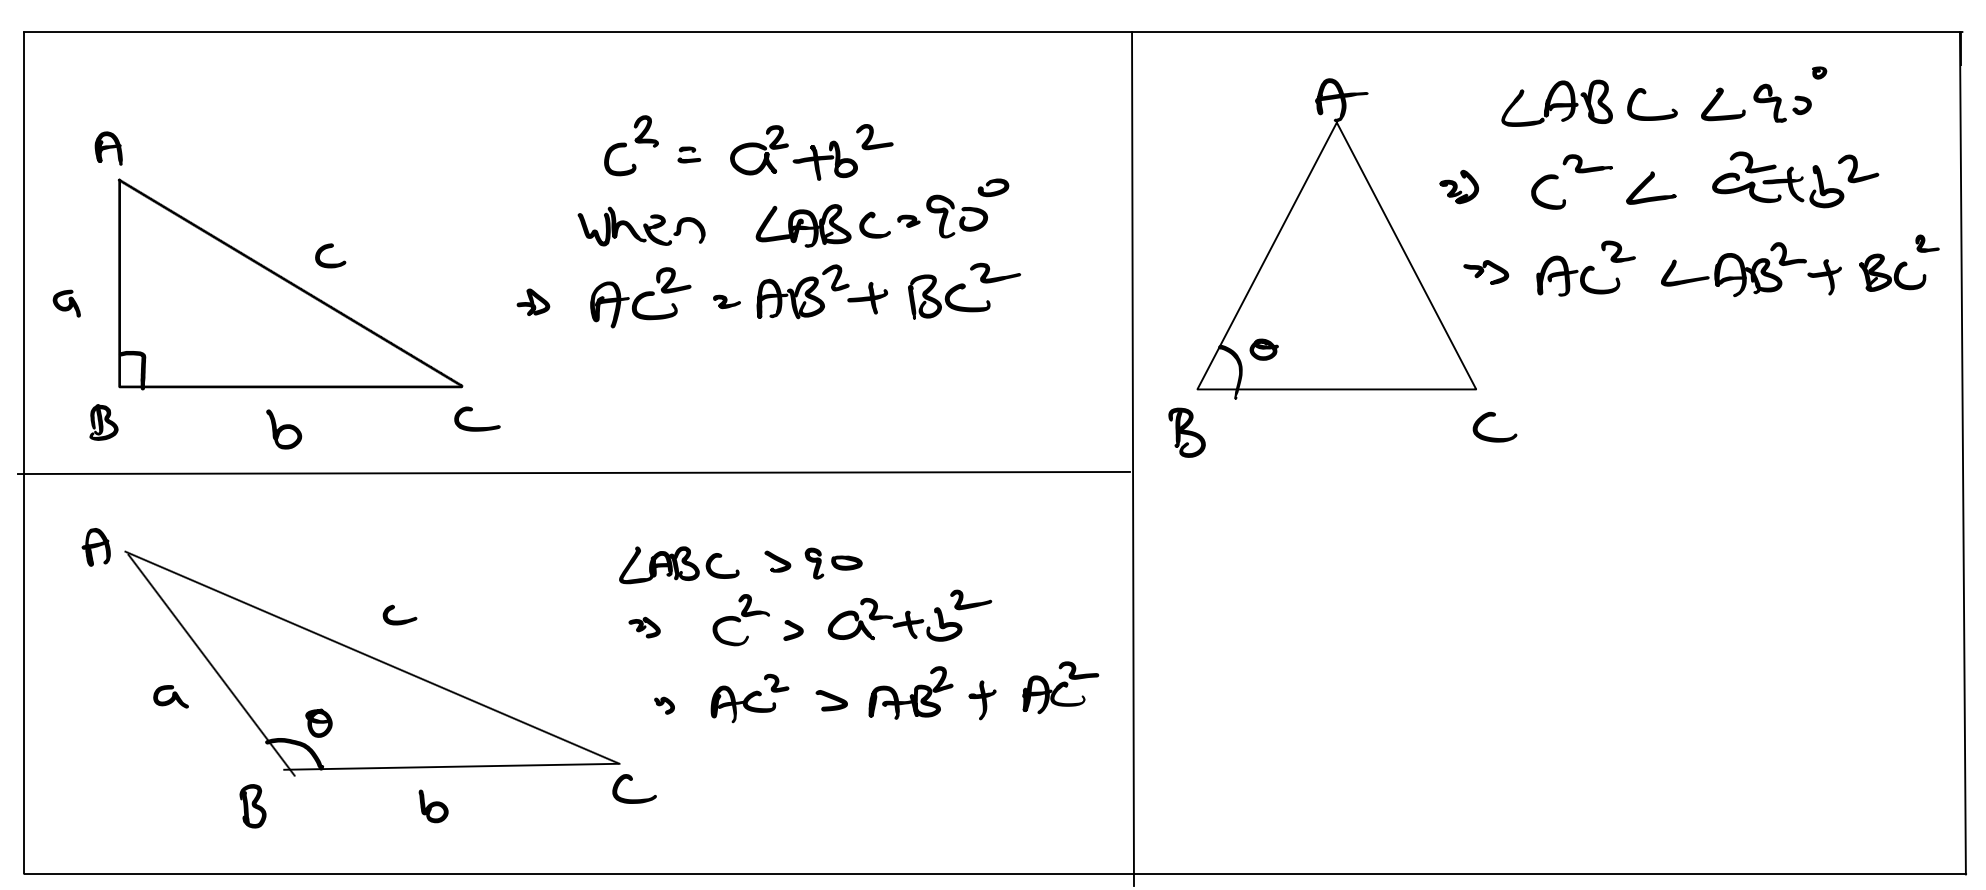
\includegraphics[width=1.0\linewidth]{Quant//Geometry//Images//Triangles/triangle_8_right_obtuse_acute_logic.png}
\end{figure}

\SampleQuestion{Determine whether a triangle with sides 12,18,23 is acute, obtuse or right}

Longest side = 23. Let use pythagoreas theorem to see how the longest side relates with other sides
\begin{align*}
    23^2 &= 12^2 + 18^2 \\
    529 &= 144 + 324 \\
    529 &> 468
\end{align*}

From above, we can conclude that the triangle is an obtuse triangle

\SampleQuestion{If 2 sides of a triangle are 8 and 15, then for how many integral values of 3rd side will the triangle will be an obtuse triangle?}

The range of values the third side can have is determined as $15 - 8 < n < 15 + 8 \implies 7 < n < 23$. We can have two scenarios

\begin{enumerate}
    \item The third side is the longest side
    \item 15 is the longest side
\end{enumerate}

In the cases below, let us assume that the third side is represented as $n$

\textbf{Case 1 : The third side is the longest side}
\begin{align*}
    n^2 &> 8^2 + 15^2 \\
    &> 64 + 225 \\
    &> 289 \\
    n &> \sqrt{289} = 17 \tag{$n$ in this case, will be a positive value only} 
\end{align*}

In this scenario, the values $n$ can take is 18,19,20,21,22

\textbf{Case 2 : 15 is the longest side}
\begin{align*}
    15^2 &> n^2 + 8^2 \\
    n^2 &< 225 - 64 \\
    n^2 &< 161 \\
    n &< \sqrt{161} \tag{$n$ in this case, will be a positive value only}
\end{align*}

In this case, the possible values $n$ can have is 8,9,10,11,12

Total values = 8,9,10,11,12,18,19,20,21,22


\newpage

















\section{Finding number of triangles when perimeter p is given}

\subsection{Nearest Integer Function (Round)}
For a decimal number $n$, the nearest integer function is represented as $\left [ n \right ]$. The behavior of this function can be seen as follows
\begin{itemize}
    \item $\Round{5.4} = 5$ : Acts as floor if value is less than 5.5
    \item $\Round{5.5} = 5$ : Acts as floor if value is equal to 5.5
    \item $\Round{5.6} = 6$ : Acts as ceil if value is greater than 5.5
\end{itemize}

\subsection{All Triangles}
\begin{equation*}
    \text{Number of triangles} = 
    \begin{cases}
        \Round{\dfrac{(p+3)^2}{48}} &\text{$p$ is odd} \\    \\
        \Round{\dfrac{p^2}{48}} &\text{$p$ is even}     
    \end{cases}
\end{equation*}

\subsection{Scalene Triangle}
In the above formula, substitute $p$ with $p-6$

\begin{equation*}
    \text{Number of triangles} = 
    \begin{cases}
        \Round{\dfrac{(p - 3)^2}{48}} &\text{$p$ is odd} \\    \\
        \Round{\dfrac{(p - 6)^2}{48}} &\text{$p$ is even}   
    \end{cases}
\end{equation*}

\subsection{Equilateral Triangle}
\begin{equation*}
    \text{Number of triangles} = 
    \begin{cases}
        0 &\text{If perimeter is not a multiple of 3}    \\
        1 &\text{If perimeter is not a multiple of 3}    \\
    \end{cases}
\end{equation*}

\subsection{Isoceles Triangle}
To get number of isoceles triangle, find count of all triangles and subtract number of scalene and isocelene triangles

\SampleQuestion{If $p = 16$, find the number of triangles that can be formed}

Since $p$ is even, the formula is $\Round{ \dfrac{p^2}{48} } \implies \Round{ \dfrac{16 * 16}{48} } = 5$

\SampleQuestion{If $p = 27$, find number of distinct triangles}
$p$ is odd therefore $\Round{ \dfrac{(p+3)^2}{48} } \implies \Round{ \dfrac{30 * 30}{48} } = 19$

\vspace{3cm}

\SampleQuestion{Find number of scalene triangles for the following values of $p$}
\begin{enumerate}
    \item 24
    \item 17
\end{enumerate}



$p = 24$ , Number of scalene triangles = $\Round{\dfrac{18 * 18}{48}} = 7$ \\

$p = 17$ , Number of scalene triangles = $\Round{\dfrac{14 * 14}{48}} = 4$

\SampleQuestion{Find number of isoceles triangle if $p=30$}

Number of isoceles triangles = all triangles - equilateral triangles - scalene triangles

\begin{itemize}
    \item All triangles : $\Round{\dfrac{30 * 30}{48}} = 19$
    \item Scalene triangles : $\Round{\dfrac{24 * 24}{48}} = 12$
    \item Equilateral triangles : 1 as 30 is divisible by 3
\end{itemize}

Isoceles triangle = $19 - 12 - 1 = 6$

\SampleQuestion{How many distinct triangles can be formed with integral sides if $p = 80$}
\begin{enumerate}
    \item With all sides even
    \item With 2 sides odd and 1 side even
\end{enumerate}

\textbf{With all sides even}
Let us assume that sides of triangle are $2a,2b,2c$. The perimeter is defined as
\begin{align*}
    2a + 2b + 2c &= 80 \\
    a + b + c &= 40
\end{align*}

Now, we can reduce the question to finding number of triangles where perimeter is 40. It is derived as $\Round{\dfrac{40 * 40}{48}} = 33$ \\

\textbf{2 sides odd and 1 side even}

\begin{WARNING}
    Let us assume that sides are $2a,2b+1,2c+1$. Perimeter is defined as $2(a+b+c+1) = 80 \implies a+b+c = 39$. Number of triangles are $\Round{\dfrac{42 * 42}{48}} = 37$ \\

    This is the wrong way of doing things. This is because for different values of $(a,b,c)$, the dimensions of triangle will be different. When we solve for the reduced triangle, then we also need to check if the values of a,b,c thus calculated also satisfy the triangle inequality for the original equation, i.e. for $2a-1, 2b-1, 2c$
\end{WARNING}

The correct way of solving this is to realise that if the perimeter of a triangle is even, it is due to following combinations only
\begin{itemize}
    \item All three even sides : $a + b + c$ where $a,b,c$ is even
    \item Two sides are odd and one is even : $a + b +c$ where $a$ is even and $b,c$ are odd
    \item We cannot have all three odd as their sum will be odd
\end{itemize}

Since we already computed values for the case where all sides are even in the above part (33), we can now find for "one odd and two even" as $all - even$ \\

Finding count of all triangles : $\Round{\dfrac{80 * 80}{48}} = 133$. "one even and two odd" is $133 - 33 = 100$

\SampleQuestion{How many distinct triangles can be formed with integral sides if perimeter is 39 with the following conditions}
\begin{enumerate}
    \item With all sides odd
    \item With 2 sides even and 1 side odd
\end{enumerate}

Let us make an observation that we made in above question. If a triangle has an odd perimeter, it can be achieved with the following combinations only
\begin{itemize}
    \item 3 odd sides
    \item 2 even sides and 1 odd side
    \item We cannot have 2 odd sides and 1 side because sum of odd sides will be even
\end{itemize}

\textbf{All sides odd}

Let sides be 2a-1, 2b-1, 2c-1. Perimeter is therefore
\begin{align*}
    2 (a + b + c) - 3 &= 39 \\
    a + b  + c &= 21
\end{align*}

For this reduce triangle, the number of triangles are $\Round{\dfrac{24 * 24}{48}} = 12$

\textbf{2 Even sides and 1 odd side}

To calculate this, we find difference of all triangles and all odd side triangles. All triangles : $\Round{\dfrac{42 * 42}{48}} = 37$. 

Answer = 37 - 12 = 25

\SampleQuestion{If perimeter of a triangle is 60, then which of the following cannot be the area of a triangle?}
\begin{enumerate}
    \item 151
    \item 159
    \item 169
    \item 176
\end{enumerate}

\textbf{For a constant perimeter $p$, maximum area of a triangle is of an equilateral triangle}. Area of equilateral triangle : $\dfrac{\sqrt{3} * a^2}{4}$ where $a$ is the side of triangle. In this case, $a = 20$. 

\begin{align*}
    \text{Area} &= \dfrac{\sqrt{3} * 20 * 20}{4} \\
    &=  100 * 1.732 \\
    &= 173.2
\end{align*}

Since the max area of the triangle can be 173.2, the option 176 can be eliminated

\newpage


















\section{Sine and Cosine Rule}
Sine and Cosine rule are relations between angles and sides of a triangle. They are explained as follows
\begin{itemize}
    \item Sine rule says that the ratio of angle and side opposite to it is equal.
    \item Cosine rule relates an angle and the three sides of a triangle 
\end{itemize}

\begin{figure}[h!]
    \centering
    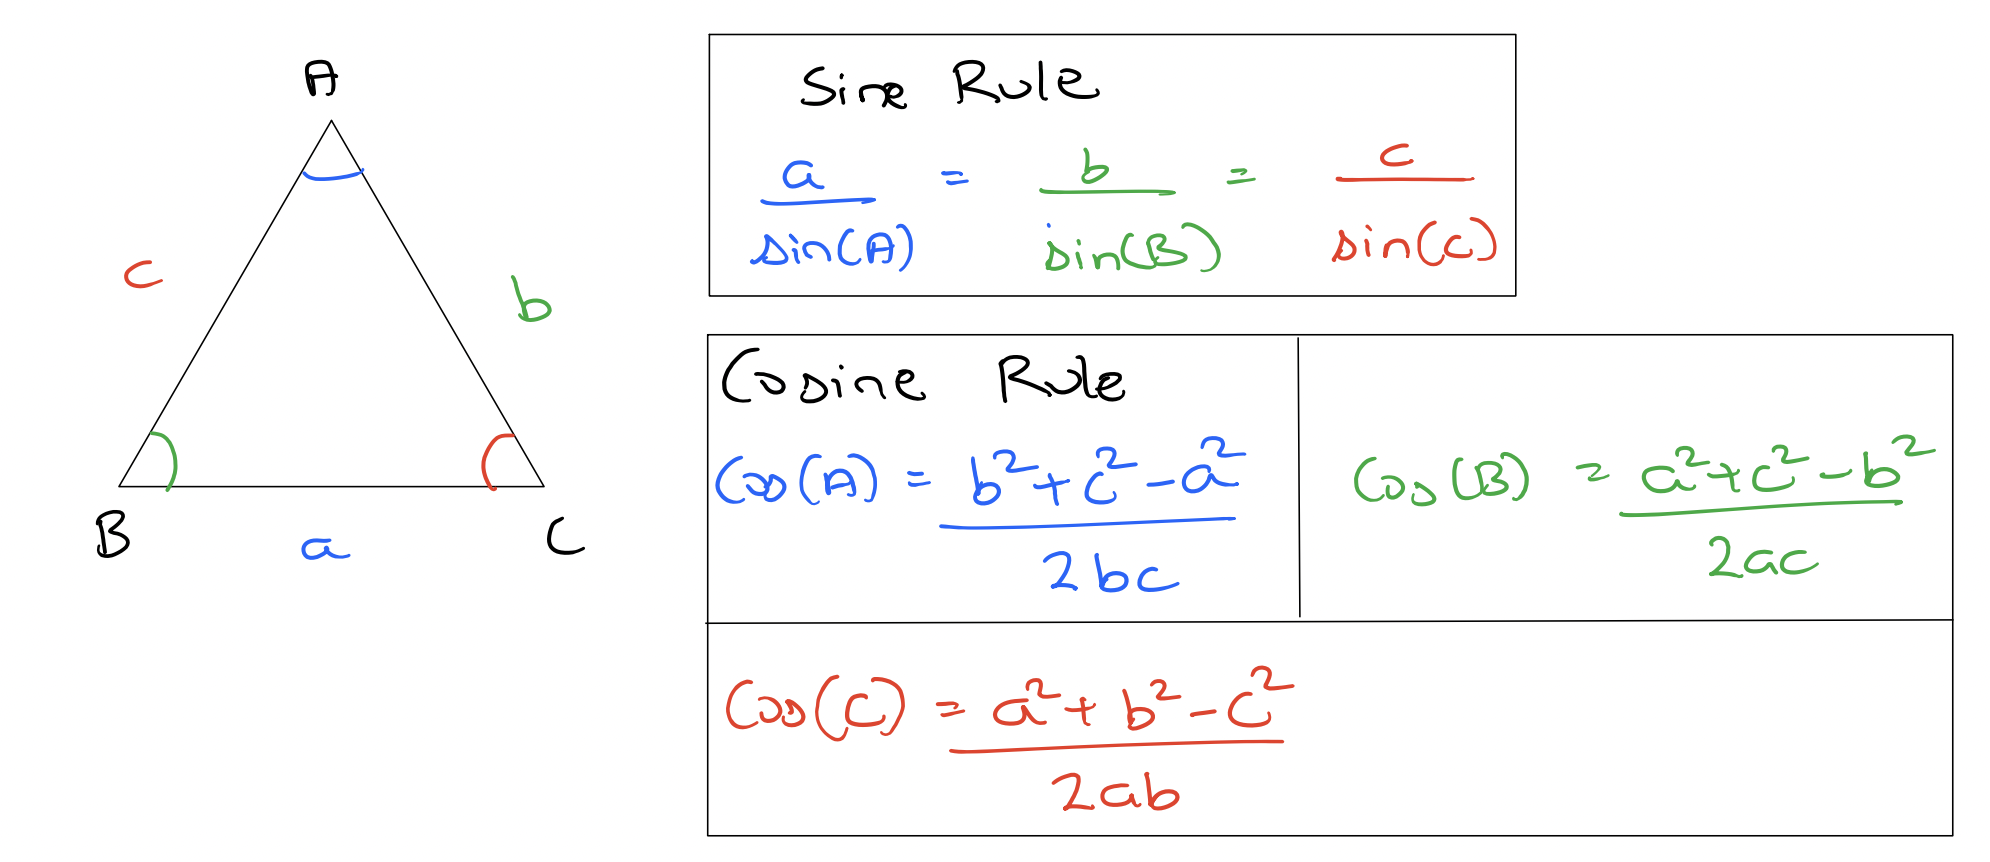
\includegraphics[width=1\linewidth]{Quant//Geometry//Images//Triangles/triangles_10_sine_and_cosine_rule.png}
\end{figure}

To apply this rule correctly, we need to understand the opposite sides and other sides. For the above $\Triangle{ABC}$, refer to the following table

\begin{table}[h!]
    \centering
    \begin{tabular}{|| c | c | c ||}
        \hline
         Angle & Opposite Side & Other Sides  \\
        \hline
         $\angle{A}$ & BC (a) & AC (b) , AB(c) \\ 
        \hline
         $\angle{B}$ & AC (b) & BC (a) , AB(c) \\ 
        \hline
         $\angle{C}$ & AB (c) & BC (a) , AC(b) \\ 
        \hline
    \end{tabular}
\end{table}

Using this, we can write sine and cosine rules as
\begin{itemize}
    \item Sine rule = $\dfrac{\text{opposite side}}{\text{angle}}$

    \item Cosine rule = $\dfrac{\text{sum of square of other sides - opposite side}}{2 * \text{product of other sides}}$
\end{itemize}

\newpage

\SampleQuestion{PM is angle bisector of $\Triangle{PQR}$ on base $QR$ and $\angle{Q} + \angle{R} = \degree{120}$. Find the length of $QR$ and $PM$}

\begin{figure}[h!]
    \centering
    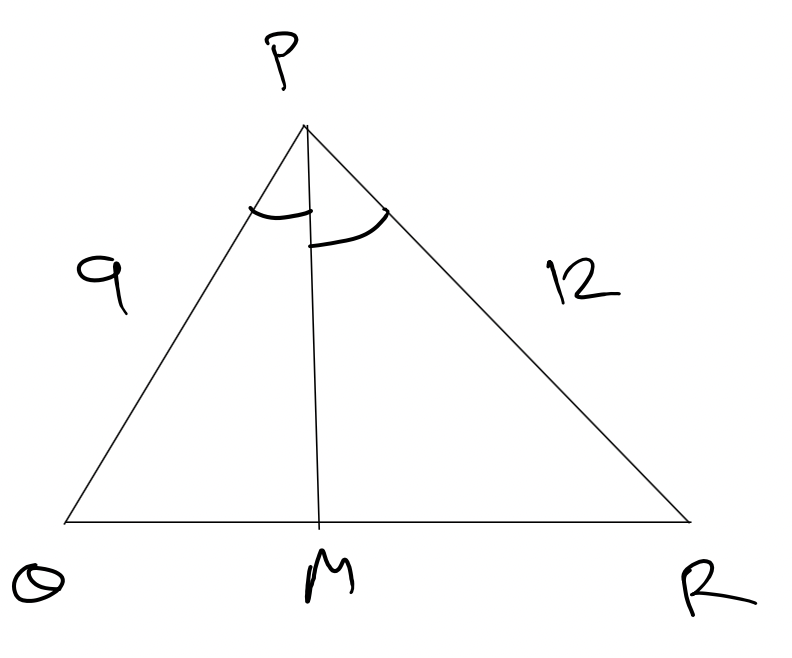
\includegraphics[width=0.35\linewidth]{./Quant/Geometry/Images/Triangles/triangle_10_question_1_img.png}
\end{figure}

\textbf{Finding QR}

To find QR, let's first find the value of $\angle{P}$ and then apply cosine rule. According to the question, $\angle{Q} + \angle{R} = \degree{120}$. This means that $\angle{P} = \degree{60}$

Applying cosine rule on $\angle{P}$
\begin{align*}
    \cos{P} &= \dfrac{12^2 + 9^2 - QR^2}{2 * 12 * 9} \\
    \cos{60} &= \dfrac{144 + 81 - QR^2}{24 * 9} \\
    \dfrac{24 * 9}{2} &= 225 - QR^2 \\
    QR &= \sqrt{225 - 108} \\
    QR &= \sqrt{117} \\
    QR &= 3 \sqrt{13}
\end{align*}

\textbf{Finding PM}
\begin{WARNING}
    PM is not perpendicular
\end{WARNING}

We can find area of PQR by adding areas of PQM and PRM. Using trigonometric formulae, we can find areas as follows
\begin{align*}
    \dfrac{PQ * PR * \sin{\angle{QPR}}}{2} &= \dfrac{PQ * PM * \sin{\angle{QPM}}}{2} + \dfrac{PM * PR * \sin{\angle{RPM}}}{2} \\
    9 * 12 * \dfrac{\sqrt{3}}{2} &= PM * (9 \sin{30} + 12 \sin{30}) \\
    54 \sqrt{3} &= \dfrac{PM}{2} * 21 \\
    PM &= \dfrac{54 * 2 * \sqrt{3}}{21} \\
    PM &= \dfrac{36 \sqrt{3}}{7}
\end{align*}

% \SampleQuestion{One of the sides of an obtuse angled isosceles triangle of perimeter 180cm is 80cm. What is the distance between incentre and circumcentre of this triangle?}

\SampleQuestion{An isoceles triangle with $\angle{P} = \degree{120}$ has an area of $16 \sqrt{3}$. What is its perimeter?}

\begin{figure}[h!]
    \centering
    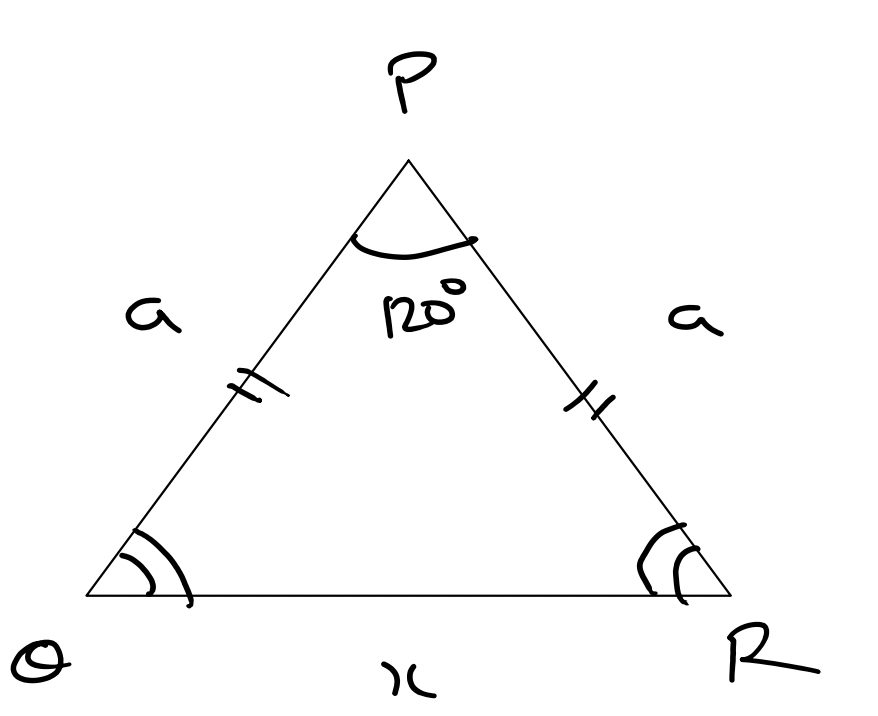
\includegraphics[width=0.5\linewidth]{Quant//Geometry//Images//Triangles/triangles_11_question_1.png}
\end{figure}

Since $\Triangle{PQR}$ is an isocles triangle, two of its sides will be equal. There is a property of isoceles triangle that if two sides are equal, then angles of those sides are equal as well. Therefore, in the above figure
\begin{itemize}
    \item PQ = PR $a$
    \item $\angle{PQR} = \angle{PRQ}$
\end{itemize}

We can understand that the value of $\angle{PQR} = \angle{PRQ} = \degree{30}$ because of the angle sum property of triangle (sum of all angles = $\degree{180}$. We now need to find the value of $a$ using area of triangle. Since we have two sides and the angle between them, we can use the trigonometric formula

\begin{align*}
    16 \sqrt{3} &= \dfrac{1}{2} * a^2 * \sin{120} \\
    32 \sqrt{3} &= a^2 * \dfrac{\sqrt{3}}{2} \tag{$\sin{(180 - x)} = \sin{x}$} \\
    a &= 8
\end{align*}

We can use sine rule to find the value of $x$ dimension. For below, we will use $\angle{PQR}$ and $\angle{QPR}$

\begin{align*}
    \dfrac{a}{\sin{30}} &= \dfrac{c}{\sin{120}} \\
    2a &= \dfrac{2}{\sqrt{3}} c \\
    c &= 8 \sqrt{3}
\end{align*}

Perimeter = $8 + 8 + 8\sqrt{3} \implies 16 + 8\sqrt{3}$

\newpage










\section{Area of triangle by ratio of sides}

\subsection{Using common height}

If two triangles share a common height and a line segment divides the base in a ration $x:y$, then we can say that the areas are divided in the ratio $x:y$ as well. In the below figure, we have $\Triangle{ABC}$ where $AD$ divides $BC$ in ratio $3:2$. $AP$ is a perpendicular. According to this, $BD = 3x, DC = 2x \implies BC = 5x$

\begin{figure}[h!]
    \centering
    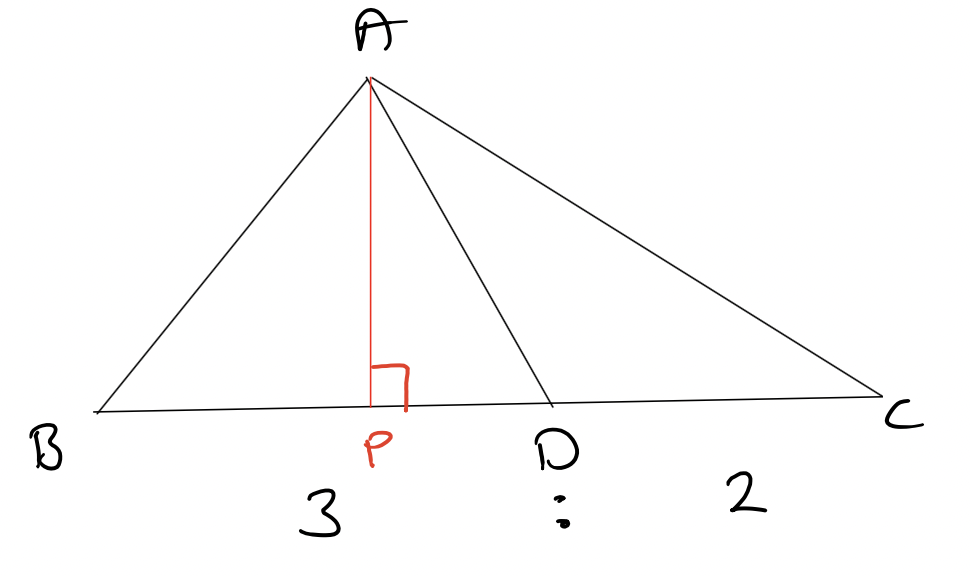
\includegraphics[width=0.4\linewidth]{Quant//Geometry//Images//Triangles/triangles_11_common_height_area.png}
\end{figure}

\begin{itemize}
    \item Area of $\Triangle{ABD}$ : The $\Triangle{ABD}$ has base $BD$ and height $AP$. The area is defined as $\frac{1}{2} * BD * AP$
    \item Area of $\Triangle{ACD}$ : The $\Triangle{ACD}$ has base $CD$ and height $AP$. The height remains same anyway, even if the height is "outside" the triangle. The area is defined as $\frac{1}{2} * CD * AP$
    \item Area of $\Triangle{ABC}$ : The $\Triangle{ABC}$ has base $BC$ and height $AP$. The area is defined as $\frac{1}{2} * BC * AP$. Since $BC = 5x$, Let us denote area of $\Triangle{ABC}$ as $5A$ where $A = \frac{1}{2} * x * AP$
    \item For area of $\Triangle{ABD}$, we can write it as $\frac{1}{2} * 3x * x * AP = 3A$
    \item For area of $\Triangle{ACD}$, we can write it as $\frac{1}{2} * 2x * x * AP = 2A$
\end{itemize}

Thus, we can see that the divided triangles have their area divided in the same ratio as well
\begin{itemize}
    \item Area$(\Triangle{ABD}) =$ $\dfrac{3}{5} \text{ Area }(\Triangle{ABC})$
    \item Area$(\Triangle{ACD}) =$ $\dfrac{2}{5} \text{ Area }(\Triangle{ABC})$
\end{itemize}

Following the above logic, we can quickly derive relationships of triangles based on their area. In the below triangle, where $BD$ divides $AC$ in ratio $2:3$

\begin{figure}[h!]
    \centering
    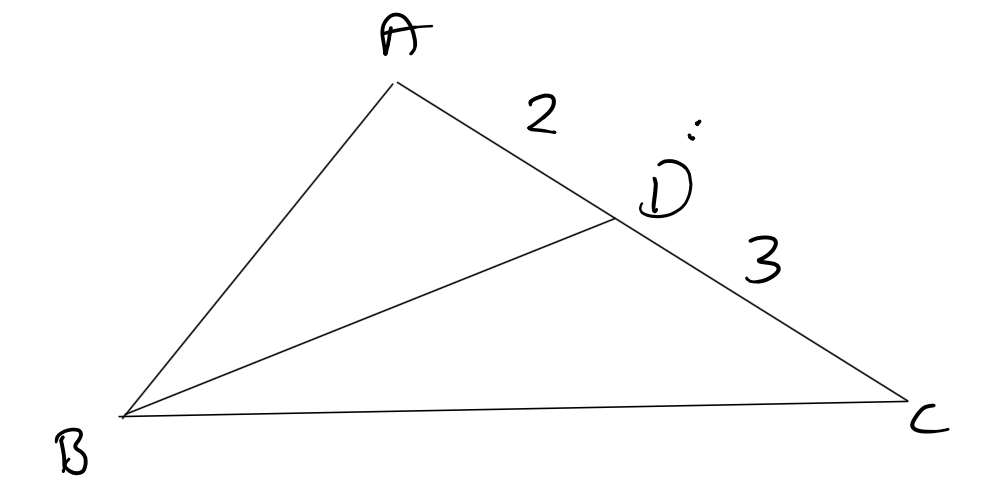
\includegraphics[width=0.4\linewidth]{Quant//Geometry//Images//Triangles/triangle_11_common_height_1.png}
\end{figure}

\begin{itemize}
    \item $\Area{\Triangle{ABD}} = \dfrac{2}{5} \Area{\Triangle{ABC}}$
    \item $\Area{\Triangle{BDC}} = \dfrac{3}{5} \Area{\Triangle{ABC}}$
\end{itemize}

\vspace{2cm}

\subsection{Using common angle}
We can also use the common angle between two triangles to find ratio of area of those triangles

\begin{figure}[h!]
    \centering
    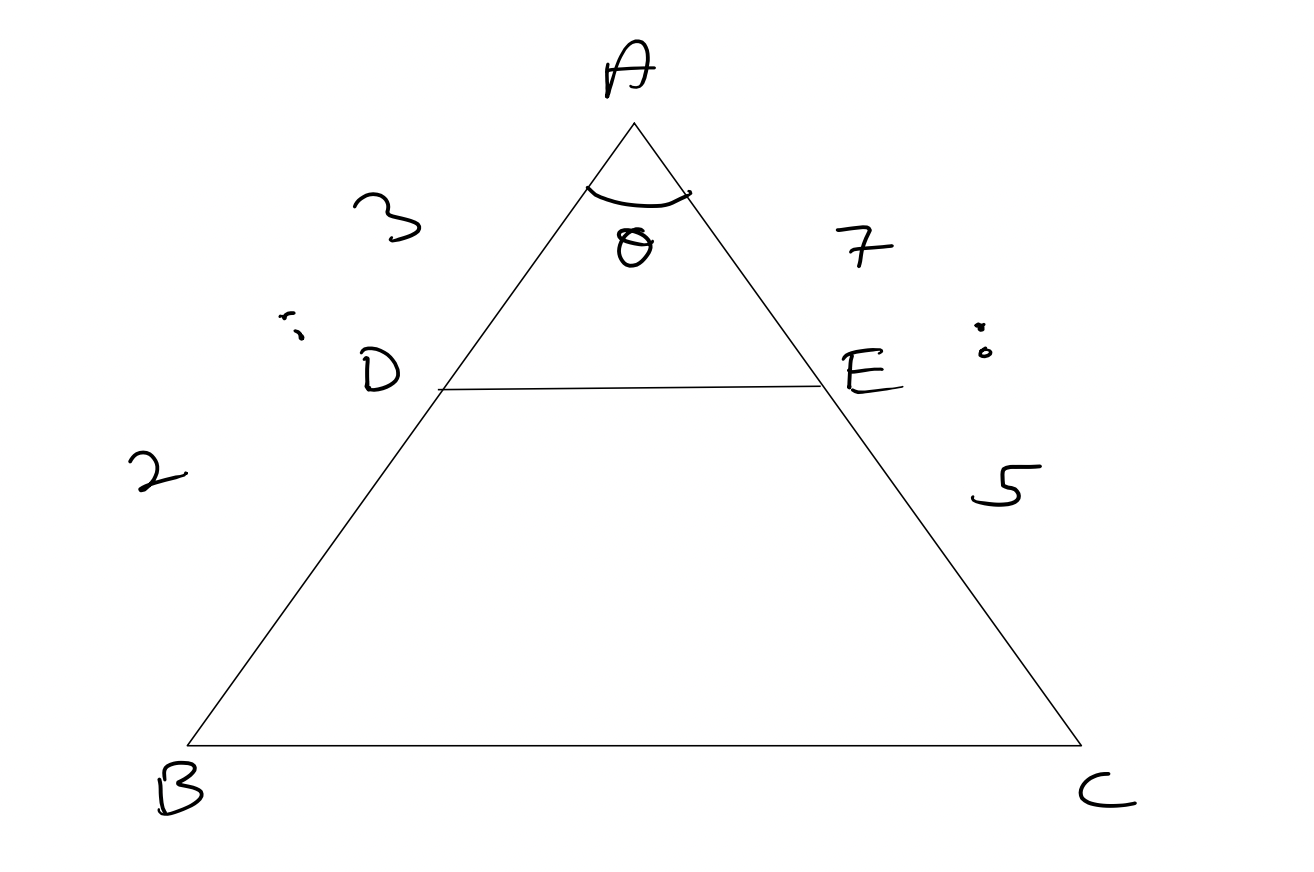
\includegraphics[width=0.5\linewidth]{./Quant/Geometry/Images/Triangles/triangle_11_common_angle_area.png}
\end{figure}

The common angle in this case is $\theta$ or $\angle{BAC}$. We can see from the figure that $AB = 5x$ and $AC = 12y$. We can find the respective areas using the formula $\dfrac{1}{2} ab \sin{\theta}$

\begin{itemize}
    \item $\Area{\Triangle{ABC}} = \dfrac{1}{2} * 5x * 12y$
    \item $\Area{\Triangle{ADE}} = \dfrac{1}{2} * 3x * 7y$
\end{itemize}

The ratio $\Area{\Triangle{ADE}}:\Area{\Triangle{ABC}} $ is
\begin{align*}
    \dfrac{\Area{\Triangle{ADE}}}{\Area{\Triangle{ABC}}} &= \dfrac{3 * 7}{5 * 12} \\
    \Area{\Triangle{ADE}} &= \dfrac{3}{5} * \dfrac{5}{12} \Area{\Triangle{ABC}} \\
    &= \dfrac{AD}{AB} * \dfrac{AE}{AC} * \Area{\Triangle{ABC}} \\
\end{align*}

\SampleQuestion{$DE$ divides $AC$ in ratio $8:5$ and $AB$ in ratio $4:3$. Find ratio of area of $ADE$ and $BDEC$}

\begin{figure}[h!]
    \centering
    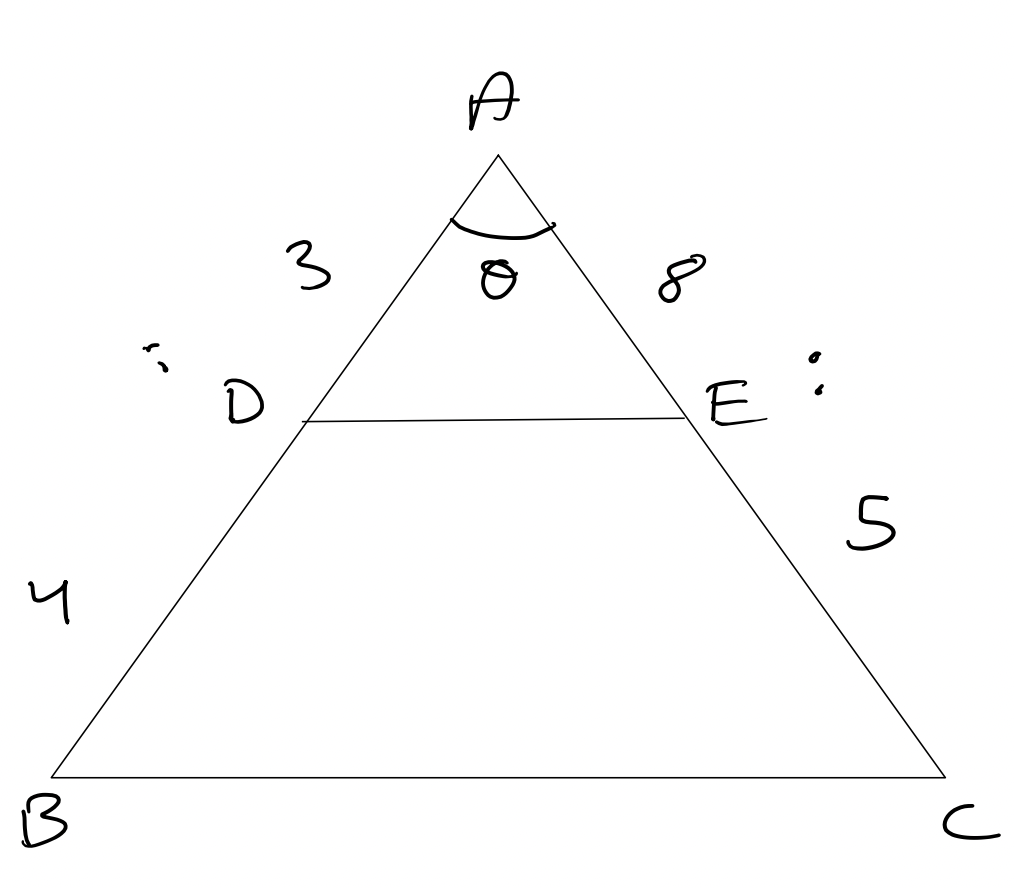
\includegraphics[width=0.3\linewidth]{Quant//Geometry//Images//Triangles/triangle_11_question_1_area.png}
\end{figure}

From our discussions above, we know that $\Area{\Triangle{ADE}} = \dfrac{3}{7} * \dfrac{8}{13} \Area{\Triangle{ABC}} \implies \dfrac{24}{91} \Area{\Triangle{ABC}}$. Using this, we can find area of quadilateral in terms of $\Triangle{ABC}$

\begin{align*}
    \Area{BDEC} &= \Area{ABC} - \dfrac{24}{91} \Area{ABC} \\
    &= \dfrac{67}{35} \Area{ABC}
\end{align*}

Ratio is therefore, $\dfrac{24 * 91}{67 * 91} = 24:67$



\SampleQuestion{DE divides AB in 5:4 and AC in 2:3. EF divides BC in 3:5. Find ratio of area of DEF and ABC}

\begin{figure}[h!]
    \centering
    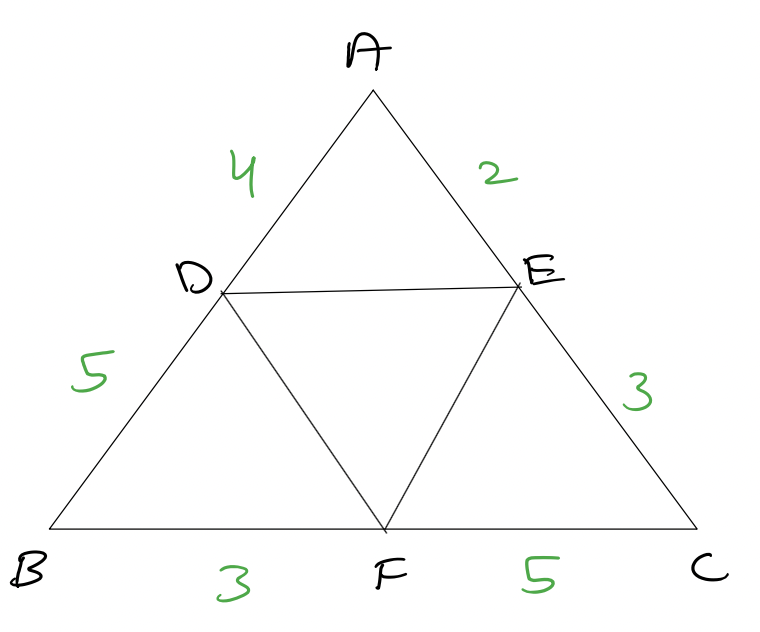
\includegraphics[width=0.5\linewidth]{Quant//Geometry//Images//Triangles/triangle_11_question_2_area.png}
\end{figure}

This is an interesting question. $\Area{DEF} = \Area{ABC} - (\Area{ADE} + \Area{BDF} + \Area{EFC})$. Using ratios, we can find $\Area{ADE},\Area{BDF},\Area{EFC}$ in terms of $\Area{ABC}$

\begin{itemize}
    \item $\Area{ADE} = \dfrac{4}{9} * \dfrac{2}{5} \Area{ABC} \impliedby \dfrac{8}{45} \Area{ABC}$
    
    \item $\Area{BDF} = \dfrac{5}{9} * \dfrac{3}{8} \Area{ABC} \impliedby \dfrac{15}{72} \Area{ABC} \implies \dfrac{5}{24} \Area{ABC}$
    
    \item $\Area{EFC} = \dfrac{3}{5} * \dfrac{5}{8} \Area{ABC} \impliedby \dfrac{3}{8} \Area{ABC}$

    \item $(\Area{ADE} + \Area{BDF} + \Area{EFC}) = \Area{ABC} * (\dfrac{8}{45} + \dfrac{5}{24} + \dfrac{3}{8}) \implies \dfrac{137}{180} \Area{ABC}$

    \item $\Area{DEF} = \Area{ABC} ( 1 - \dfrac{137}{180} ) \implies \dfrac{43}{180} \Area{ABC} \implies \Area{DEF} : \Area{ABC} = 43:180$

\end{itemize}

\newpage




\section{Midpoint Theorem and Proportionality Theorem}

\subsection{Midpoint Theorem}
In a triangle, if from the midpoint of a triangle, a parallel line is drawn to other side of the triangle such that it is parallel with a side of triangle, the endpoint of the newly drawn line will be a midpoint to the other side and the length of this parallel line will be half of the side it is parallel with \\

In below figure, D is a midpoint of AB. We have drawn DE, which is parallel to BC. The vertex E acts as the midpoint of line AC

\begin{figure}[h!]
    \centering
    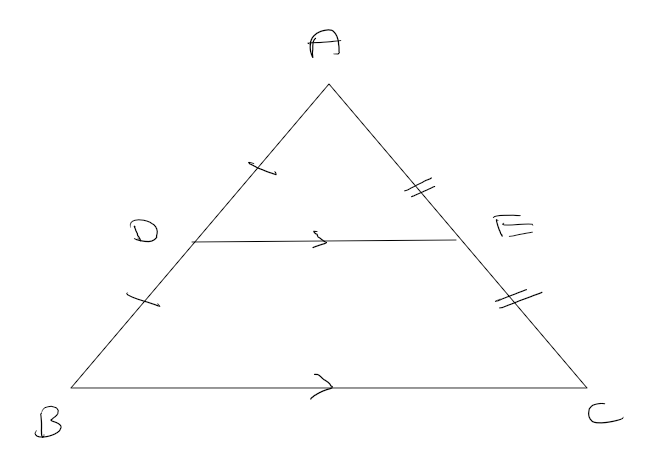
\includegraphics[width=0.5\linewidth]{Quant//Geometry//Images//Triangles/triangle_12_midpoint_theorem_result.png}
\end{figure}

The basis of this property is similarity of triangles. In the above figure, we can easily prove that $\Triangle{ADE}$ is similar to $\Triangle{ABC}$ by AA similarity condition. In similar triangles, ratio of sides is equal. If D is the midpoint of AB then $\dfrac{AD}{AB} = \dfrac{1}{2}$. Using the rules of similarity, $\dfrac{AD}{AB} = \dfrac{DE}{BC} = \dfrac{AE}{AC} = \dfrac{1}{2}$. Thus
\begin{itemize}
    \item E is midpoint of AC as $\dfrac{AE}{AC} = \dfrac{1}{2}$
    \item $DE = \dfrac{1}{2} BC$ as $\dfrac{DE}{BC} = \dfrac{1}{2}$
\end{itemize}

\SampleQuestion{In the figure below, BC = 16 and AM = 12. N is midpoint of AC and T is midpoint of BM. AM is perpendicular to BC. Find the length of TN}

\begin{figure}[h!]
    \centering
    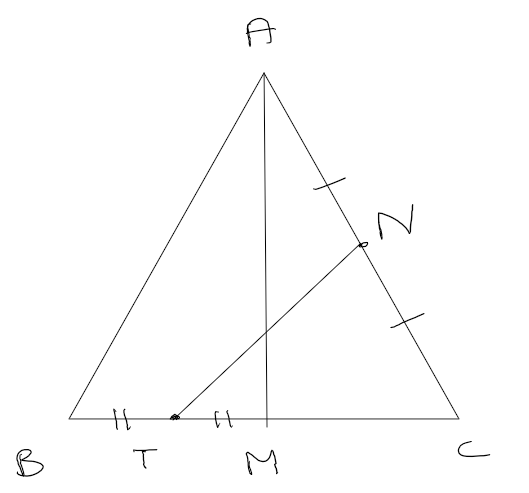
\includegraphics[width=0.35\linewidth]{Quant//Geometry//Images//Triangles/triangle_12_midpt_question_1.png}
\end{figure}

A general rule to remember is that whenever we have to find the length of a line that is not either perfectly vertical or horizontal, we can use pythagoreas theorem. We can split any "angled" line into a horizontal and vertical component, find those lengths and then use pythagoreas theorem to find the actual length. In the triangle, we can create a line NR parallel to AM on BC. 

\begin{figure}[h!]
    \centering
    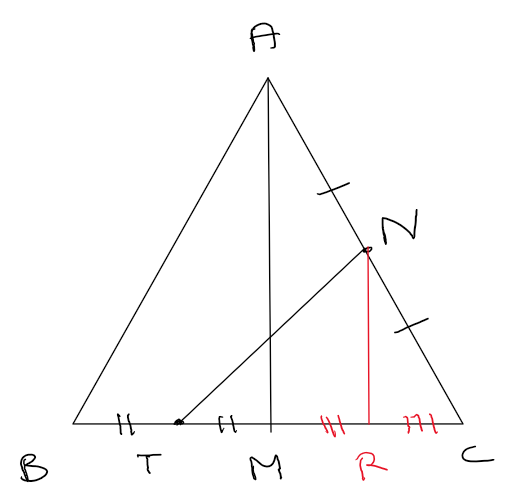
\includegraphics[width=0.35\linewidth]{Quant//Geometry//Images//Triangles/triangle_12_midpoint_q1_ans_1.png}
\end{figure}

Since NR is parallel to AM (and also perpendicular. Any line that is parallel to a perpendicular is a perpendicular itself), we can apply midpoint theorem and say that R is the midpoint of MC. Also, NR = $\dfrac{AM}{2} \implies \dfrac{12}{2} = 6$ because of midpoint theorem as well. \\

To calculate TN, we now need TR as well so that we can apply pythagoreas theorem. We can see that 
\begin{align*}
    BC &= BM + MC \\
    16 &= BT + TM + MR + CR \\
    16 &= 2 (TM + MR) \tag{BT = TM and MR = CR} \\
    TM + MR &= 8 \\
    TR &= 8 \tag{TM + MR = TR}
\end{align*}

Now, we can apply pythagoreas theorem in $\Triangle{NTR}$ and we will get $TN = 10$

\newpage
\SampleQuestion{In the below figure, P is the midpoint of AN and N is the midpoint of BC. Answer the following}
\begin{itemize}
    \item Find $AQ : QC$
    \item If $\Area{\Triangle{ABC}} = 120$, find $\Area{\Triangle{APQ}}$
\end{itemize}

\begin{figure}[h!]
    \centering
    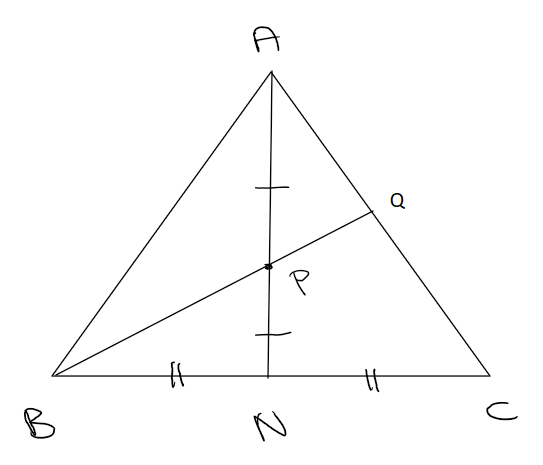
\includegraphics[width=0.35\linewidth]{Quant//Geometry//Images//Triangles/triangle_12_midpt_q2_img.png}
\end{figure}

We need to find someway through which we can get a relation between AQ and QC. Since N and P are midpoints, we can use midpoint theorem to simplify our work. In $\Triangle{BQC}$, we can apply midpoint theorem by constructing a line NR which is parallel to BQ. Because of this, QC will be split into two equal parts QR and CR

\begin{figure}[h!]
    \centering
    \includegraphics[width=0.35\linewidth]{Quant//Geometry//Images//Triangles/triangle_12_midpt_q2_ans_image_1.png}
\end{figure}

We can also determine that if NR is parallel to BQ, then it must be parallel to PQ as well as PQ is a part of BQ. Therefore, in $\Triangle{ANR}$, according to midpoint theorem, Q is midpoint of AR meaning AQ = AR. 
\begin{align*}
    AC &= AQ + QR + CR \\
    &= 3 AQ \tag{AQ = QR and QR = RC as proved above} \\
    AQ &= \dfrac{1}{3} AC
\end{align*}

From above, we can see that $QC = \dfrac{AC}{2}$ and thus, $AQ : QC = 1 : 2$ \\

If area of $\Triangle{ABC}$ is 120, then we can say that $\Area{ANC} = 60$ as N is midpoint of BC. We can zoom in on $\Triangle{ANC}$ and observe that Q divides AC into two sides of ratio $1 : 2$ (AQ : QC). Similarly, P divides AN in two equal parts. According to what we discussed about triangles having common height and ratio of sides, $\Area{\Triangle{APQ}} = \dfrac{1}{2} * \dfrac{1}{3} * \Area{\Triangle{ANC}} \implies \dfrac{60}{6} = 10$

\newpage

\subsection{Proportionality Theorem}

If 2 parallel lines are intersected at different points by transversals from the same point, then the ratio of those segments are equal.

\begin{figure}[h!]
    \centering
    \includegraphics[width=0.6\linewidth]{Quant//Geometry//Images//Triangles/triangle_12_proportionality_theorem_img.png}
\end{figure}

In the above figure, $PQ || XY$ (PQ is parallel to XY) and we have three transversals AC, AH and AS all originating from same point A. According to the theorem, $\dfrac{AB}{BC} = \dfrac{AG}{GH} = \dfrac{AR}{RS}$

\SampleQuestion{In the below figure, AE = 14, ED = 10, DC = 12, CA = 16, $AB : BC = 3 : 5$. Find the area of the shaded region $\Triangle{EFD}$}
\begin{figure}[h!]
    \centering
    \includegraphics[width=0.5\linewidth]{Quant//Geometry//Images//Triangles/triangle_12_midpt_propo_q1.png}
\end{figure}

This is an interesting question. We can find the dimension AD using concept of pythagorean triplets (or simply applying pythagoreas theorem). The triplet in $\Triangle{ACD}$ resembles (3,4,5) with a multiplier of 4 $\implies$ (12,16,20). Therefore, AD = 20 \\

Since DC and EB are parallel, we can see that a vertex A has two transversals AC and AD intersecting these lines. According to proportionality theorem, $\dfrac{AB}{BC} = \dfrac{AF}{FD} = \dfrac{3}{5}$. In $\Triangle{AED}$, the line EF divides AD in ratio $3 : 5$. Therefore, $\Area{\Triangle{EFD}} = \dfrac{5}{8} * \Area{\Triangle{AED}}$ \\

Using heron's formula, we will calculate $\Area{\Triangle{AED}}$
\begin{align*}
    s &= \dfrac{14 + 10 + 20}{2} = 22 \\
    \Area{\Triangle{AED}} &= \sqrt{22 * (22 - 20) * (22 - 10) * (22 - 14)} \\
    &= \sqrt{(2 * 11) * (2) * (2 * 2 * 3) * (2 * 2 * 2)} \\
    &= \sqrt{2^7 * 3 * 11} \\
    &= 8 \sqrt{66}
\end{align*}

$\Area{\Triangle{FED}} = \dfrac{8 * 5 \sqrt{66}}{8} = 5 \sqrt{66}$

\newpage











\section{Equilateral Triangles}
In an equilateral triangle, we have the following properties
\begin{itemize}
    \item All sides are equal (represented as $a$ in below figure)
    \item All angles are $\degree{60}$
    \item Centroid , Orthocenter , Incenter and Circumcenter are at the same point
    \item Median is perpendicular to the base $\implies$ median is a perpendicular bisector
\end{itemize}

\begin{figure}[h!]
    \centering
    \includegraphics[width=0.5\linewidth]{Quant//Geometry//Images//Triangles/triangle_13_equilateral_theory.png}
\end{figure}

Using the above figure, we can derive some results
\begin{itemize}
    \item Height
    \begin{itemize}
        \item D is a midpoint of BC $\implies BD = \dfrac{a}{2}$
        \item Taking BD as base in $\Triangle{ABD}$, we can find height AD as $\dfrac{AD}{BD} = \tan{\degree{60}} \implies AD = \dfrac{\sqrt{3} a}{2}$
    \end{itemize}

    \item Area : Using $\dfrac{1}{2} * \text{ base } * \text{ height }$ formula, we get $\dfrac{1}{2} * a * \dfrac{a \sqrt{3}}{2} = \dfrac{\sqrt{3} a^2}{4}$

    \item Inradius and Circumradius
    \begin{itemize}
        \item AD is a median and O is a centroid. Therefore, $AO : OD = 2 : 1$. Now, $OD$ is inradius and $OA$ is circumradius $\implies \dfrac{R}{r} = 2$
        \item Relating with height, we get $r = \dfrac{1}{3} * \dfrac{\sqrt{3} a}{2} \implies \dfrac{a}{2 \sqrt{3}}$
        \item Relating with height, we get $R = \dfrac{2}{3} * \dfrac{\sqrt{3} a}{2} \implies \dfrac{a}{\sqrt{3}}$
    \end{itemize}
\end{itemize}
\newpage

\SampleQuestion{There is an equilateral triangle with side of 2 units. A circle is inscribing it and another circle is circumscribing it. The circle circumscribing it is inscribed inside another equilateral triangle as shown in the figure below. Find the area of the bigger equilateral triangle}

\begin{figure}[h!]
    \centering
    \includegraphics[width=0.5\linewidth]{Quant//Geometry//Images//Triangles/triangle_13_q1.png}
\end{figure}

We can use the above results to easily calculate this. For the inner triangle, all measurements will have a subscript of $i$ and for outer triangle, a subscript of $o$. For example, side of inner triangle is $a_i$ and outer triangle is $a_o$

\begin{itemize}
    \item $R_i = \dfrac{a_i}{\sqrt{3}}$
    \item The circumradius of inner triangle is the inradius of the bigger triangle $\implies r_o = R_i$
\end{itemize}

\begin{align*}
    r_o &= \dfrac{a_o}{2 \sqrt{3}} \\ 
    \dfrac{a_i}{\sqrt{3}} &= \dfrac{a_o}{2 \sqrt{3}} \\
    a_o &= 2 a_i \\
    a_o &= 4 \tag{$a_i = 4$ is given}
\end{align*}

Area of outer triangle : $\dfrac{\sqrt{3} * 16}{4} = 4 \sqrt{3}$
